\documentclass[12pt,a4paper]{article}
\usepackage{solutions}
\usepackage{multicol}
\usepackage{float}
\usepackage{todonotes}

\title{Домашнее задание от 12.10.\\Теоретическая информатика. 2 курс.\\Решения.}
\author{Глеб Минаев @ 204 (20.Б04-мкн)}
% \date{}

\newcommand{\RE}{\mathrm{RE}}
\newcommand{\Insertion}{\mathrm{Insertion}}
\newcommand{\Insertioncirc}{\mathrm{Insertion}^\circ}

\begin{document}
    \maketitle

    \begin{multicols}{2}
        \tableofcontents
    \end{multicols}

    \begin{problem}{3}\ 
        \begin{enumerate}
            \renewcommand{\labelenumi}{(\theenumi)}
            \renewcommand{\theenumi}{\alph{enumi}}
            \item Давайте рассмотрим грамматику с правилами
                \begin{align*}
                    S &\to P'aB,&
                    P' &\to \varepsilon \mid P&
                    P &\to aP \mid bPa \mid ba,&
                    B &\to b \mid bA,&
                    A &\to aA \mid B.
                \end{align*}

                Для начала заметим, что $B$ порождает язык слов над $\{a; b\}$, начинающихся и заканчивающихся на $b$, т.е.
                \[\{b a^{n_1} b \dots b a^{n_k} b \mid k \geqslant 0 \wedge n_1, \dots, n_k \geqslant 0\},\]
                а $A$ --- только заканчивающихся на $b$, т.е.
                \[\{a^{n_1} b \dots b a^{n_k} b \mid k \geqslant 0 \wedge n_1, \dots, n_k \geqslant 0\}.\]
                Действительно, покажем это по индукции по $|w|$ (одновременно и для $A$ и для $B$).
                \begin{itemize}
                    \item Если $|w| = 0$, то $w$ не может быть порождена. Действительно, все замены $B$ создают новый символ, а единственная замена $A$, не создающая нового символа --- $A \to B$, т.е. в итоге хотя бы один символ будет порождён.
                    \item Пусть $w$ была порождена $B$. Если первым шагом была проведена замена $B \to b$, то $w = b$, что верно (или просто не может быть, если $|w| \neq 1$). Иначе первым шагом было получено $bA$, т.е. $w = bu$, где $u$ была порождена $A$, откуда по предположению индукции сразу следует требуемое.
                    \item Пусть $w$ была порождена $A$. Если первым шагом была проведена замена $A \to B$, то $w$ порождена $B$, а тогда мы уже показали, что получится, что надо. Иначе первым шагом было получено $aA$, т.е. $w = au$, где $u$ была порождена $A$, откуда по предположению индукции сразу следует требуемое.
                    \item Теперь пусть дана строка
                        \[w \in \{b a^{n_1} b \dots b a^{n_k} b \mid k \geqslant 0 \wedge n_1, \dots, n_k \geqslant 0\}.\]
                        $|w| = 0$ быть не может. Если $|w| = 1$, то $w = b$, а тогда $w$ получается из $B$ заменой $B \to b$. Иначе $w = bu$ и
                        \[u \in \{a^{n_1} b \dots b a^{n_k} b \mid k \geqslant 0 \wedge n_1, \dots, n_k \geqslant 0\}.\]
                        Тогда по предположению индукции $u$ порождается $A$, а тогда $w$ будет порождена заменой $B \to bA$, где $A$ будет разобрана по дереву разбора $u$.
                    \item Теперь пусть дана строка
                        \[w \in \{a^{n_1} b \dots b a^{n_k} b \mid k \geqslant 0 \wedge n_1, \dots, n_k \geqslant 0\}.\]
                        $|w| = 0$ быть не может. Если $w = bu$ и
                        \[u \in \{a^{n_1} b \dots b a^{n_k} b \mid k \geqslant 0 \wedge n_1, \dots, n_k \geqslant 0\}.\]
                        Тогда по предположению индукции $u$ порождается $A$, а тогда $w$ будет порождена заменой $A \to B$, затем $B \to bA$, где $A$ будет разобрана по дереву разбора $u$. Иначе $w = au$ и
                        \[u \in \{a^{n_1} b \dots b a^{n_k} b \mid k \geqslant 0 \wedge n_1, \dots, n_k \geqslant 0\}.\]
                        Тогда по предположению индукции $u$ порождается $A$, а тогда $w$ будет порождена заменой $A \to aA$, где $A$ будет разобрана по дереву разбора $u$.
                \end{itemize}

                Теперь заметим, что $P$ порождает язык
                \[\{a^{n_1} b \dots b a^{n_k} \mid k \geqslant 2 \wedge n_1, \dots, n_k \geqslant 0 \wedge n_k = k-1\}.\]
                Давайте переосмыслим, что это за язык. Всякую строку (из $\{a; b\}^*$) имеет вид $a^{n_1} b \dots b a^{n_k}$ для некоторых $k \geqslant 1$ и $n_1, \dots, n_k \geqslant 0$. Т.е. условия $k \geqslant 2$ и $n_1, \dots, n_k \geqslant 0$ говорят лишь, что в строке есть хотя бы один символ $b$. Но! Блок символов $a^{n_i}$ --- это блок между двумя соседними $b$-шками, что слева от неё $i-1$ $b$-шка. Т.е. условие $n_k = k-1$ говорит, что после последней $b$-шки идёт столько $a$-шек, сколько $b$-шек во всей строке.
                
                Пусть какая-то сентенциальная форма была получена из $P$. Очевидно, что она имеет вид $vPu$ или вид $w$, где $v, w \in \{a; b\}^*$, $u \in a^*$. Для начала покажем по индукции по $|v| + |u|$, что $|u|=|v|_b$.
                \begin{itemize}
                    \item Действительно, когда $|v| + |u| = 0$, то условие очевидно.
                    \item Тогда пусть сентенциальная форма $vPu$ получена из $P$, а $|v| + |u| > 0$. Тогда последним была применена одна из замен $P \to aP$ и $P \to bPA$. Если первая, то $v = v' a$, а $u = u'$, иначе $v = v' b$, а $u = a u'$. Тогда $v' P u'$ --- другая сентенциальная форма, порождённая из $P$, а $|v'| + |u'| < |v| + |u|$. Тогда по предположению индукции $|v'|_b = |u'|$. Отсюда сразу следует, что $|v|_b = |u|$.
                \end{itemize}
                Также заодно покажем по индукции по $|v| + |u|$, что для всякой пары $(v; u)$, где $v \in \{a; b\}^*$, $u \in a^*$, $|v|_b = |u|$, сентенциальная форма $vPu$ будет порождена $P$.
                \begin{itemize}
                    \item Если $|v| + |u| = 0$, то $vPu = P$.
                    \item Если $|v| + |u| > 0$, то либо $|v| > 0$, либо $|u| > 0$. При этом $|v| \geqslant |v|_b = |u|$, а значит $|v| > 0$ в любом случае. Тогда если $v = v' a$, то $|v'|_b = |v|_b = |u|$, а значит $v' P u$ будет порождена $P$, откуда $vPu$ получается заменой $P \to aP$. Если же $v = v'b$, тогда $|u| > 0$, а значит $u = a u'$. Тогда $|v'|_b = |v|_b - 1 = |u| - 1 = |u'|$, а значит $v'Pu'$ порождается $P$, откуда $vPu$ будет порождена заменой $P \to bPa$. 
                \end{itemize}
                Теперь заметим, что если слово $w$ было порождено $P$, то последней заменой была $P \to ba$, а $w$ получилась из сентенциальной формы $vPu$ с описанными выше условиями, т.е.
                \[w \in \{a^{n_1} b \dots b a^{n_k} \mid k \geqslant 2 \wedge n_1, \dots, n_k \geqslant 0 \wedge n_k = k-1\}.\]
                При этом для всякой такой строки $w$ верно, что она имеет вид $vbau$, где $v \in \{a; b\}^*$, $u \in a^*$, $|v|_b = |u|$, а значит $vPu$ порождается из $P$, а $w$ из неё заменой $P \to ba$. Следовательно, мы доказали, что именно этот язык порождается из $P$.

                Отсюда легко видеть, что из $P'$ порождается язык
                \[\{a^{n_1} b \dots b a^{n_k} \mid k \geqslant 1 \wedge n_1, \dots, n_k \geqslant 0 \wedge n_k = k-1\},\]
                а значит из $P'a$ порождается язык
                \[\{a^{n_1} b \dots b a^{n_k} \mid k \geqslant 1 \wedge n_1, \dots, n_k \geqslant 0 \wedge n_k = k\}.\]
                Следовательно, понятно, что из $S$ порождается язык
                \[\{a^{n_1} b \dots b a^{n_k} b \mid k \geqslant 1 \wedge n_1, \dots, n_k \geqslant 0 \wedge n_i = i \text{ для некоторого $i$}\}.\]

            \item Сразу заметим, что этот язык сожно также записать как
                \[\{aba^2b \dots a^n b \mid n \geqslant 1\}.\]
                Отсюда понятно, что если в слове из данного языка $n$ букв $b$, то в нём $\frac{n(n+1)}{2}$ символов $a$, т.е. $\frac{|w|_a}{|w|_b} \to \infty$ при $|w| \to \infty$. Пусть дано $p > 0$. Возьмём любое слово $w$ в нашем языке длины хотя бы $p$. Пусть дано некоторое разбиение $w = pxqyr$, что $p, q, r, x, y \in \{a; b\}^*$, $|xqy| \leqslant p$, $|xy| > 0$. Тогда
                \[|p x^d q y^d r|_a = |pxqyr|_a + (d-1)(|x|_a + |y|_a), \qquad |p x^d q y^d r|_a = |pxqyr|_b + (d-1)(|x|_b + |y|_b).\]
                А значит если $|x|_b + |y|_b > 0$, то
                \[\lim_{d \to \infty} \frac{|p x^d q y^d r|_a}{|p x^d q y^d r|_b} = \frac{|x|_a + |y|_a}{|x|_b + |y|_b} < \infty.\]
                Следовательно, какая-то подпоследовательность слов $p x^d q y^d r$ не лежит в нашем языке. Если же $|x|_b + |y|_b = 0$, то $|p x^d q y^d r|_b = |pxqyr|_b$, но
                \begin{align*}
                    |p x^d q y^d r|_a
                    &= |pxqyr|_a + (d-1)(|x|_a + |y|_a)\\
                    &= \frac{|pxqyr|_b(|pxqyr|_b + 1)}{2} + (d-1)(|x|_a + |y|_a)\\
                    &\neq \frac{|px^dqy^dr|_b(|px^dqy^dr|_b + 1)}{2}.
                \end{align*}
                Следовательно, слова $p x^d q y^d r$ для всякого $d \neq 1$ не лежат в языке.

            \item Давайте рассмотрим грамматику с правилами
                \begin{align*}
                    S &\to L'aR'b,&
                    L' &\to \varepsilon \mid L&
                    L &\to aL \mid bLa \mid ba,&
                    R' &\to \varepsilon \mid R,&
                    R &\to Ra \mid aRb \mid ab.
                \end{align*}

                Заметим, что $L$ и $L'$ замкнуты на себе (т.е. из нетерминальных символов порождают только $L$ и $L'$) и имеют правила аналогичные $P'$ и $P$ из пункта (a) соответственно. Значит $L$ порождает язык
                \[\{a^{n_1} b \dots a^{n_k} b a^k \mid k \geqslant 0 \wedge n_1, \dots, n_k \geqslant 0\} =: M_L.\]
                $R$ и $R'$ работают аналогично, но только развёрнуто, поэтому $R$ порождает язык
                \[\{a^k b a^{n_1} \dots b a^{n_k} \mid k \geqslant 0 \wedge n_1, \dots, n_k \geqslant 0\} =: M_R.\]
                Следовательно задача остаётся за тем, чтобы понять, почему $M_L a M_R b$ --- этот тот язык, который нам нужен.

                Несложно, видеть, что $M_L$ --- этот язык строк $a^{n_1} b \dots a^{n_k} b a^k$, а $a M_R b$ --- строк $a^{m_1} b \dots a^{m_l} b$, где $m_1 = l$. Тогда склеивая эти строчки получаем строчку вида $a^{p_1} b \dots a^{p_s} b$, где $s = k + l$, a $p_{k+1} = k + m_1 = k + l = s$, т.е. язык $M_L a M_R b$ является подмножеством искомого.

                При этом если дана строка $w = a^{n_1} b \dots a^{n_k} b$, где $k \geqslant 1$, а $n_i = k$, то тогда
                \begin{gather*}
                    v := a^{n_1} b \dots a^{n_{i-1}} b a^{i-1} \in M_L,\\
                    u := a^{k-i} b a^{n_{i+1}} \dots b a^{n_k} \in M_R,
                \end{gather*}
                и при этом $w = uavb$, так как $a^{i-1} a a^{k-i} = a^k = a^{n_i}$. Следовательно искомый язык является подмножеством $M_L a M_R b$.
        \end{enumerate}
    \end{problem}

    \begin{problem}{4}
        \newcommand{\Substrings}{\mathrm{Substrings}}
        \newcommand{\Postfix}{\mathrm{Postfix}}
        \newcommand{\Prefix}{\mathrm{Prefix}}
        \newcommand{\Rev}{\mathrm{Rev}}
        Пусть имеется грамматика $(\Sigma, N, R, S)$. Сначалаа почистим её: бывают иногда плохие нетерминальные символы, когда не могут породить ни одного слова (например, если у символа $P$ есть только правило $P \to PP$). Для этого просто удалим нетерминальные символы, которые не могут породить ни одного слова, а вместе с ними удалим правила, в которых они встречаются. Если $S$ --- был таким непорождающим символом, то грамматика не порождает ни одного слова (а тогда она неинтересна: задача для неё очевидна). Значит $S$ всё ещё будет определено, а $\Sigma$ не поменяется, т.е. мы действительно получили грамматику. Заметим, что если какое-то слово порождался каким нибудь нетерминальным символом (не обязательно $S$), то в его дереве разбора нет непорождающих нетерминальных символов (так как иначе поддерево этого символа будет способом порождения некоторого слова из данного символа). Следовательно, всё, что порождалось раньше, порождается и сейчас. Ну а так как мы убрали правила и не добавляли новых, то всё, что порождается сейчас, порождалось раньше. Теперь мы готовы начинать.
        
        Рассмотрим грамматику $(\Sigma, N', R', S')$, где
        \begin{itemize}
            \item $N' := N \cup \{T_A\}_{A \in N}$, где $T_A$ --- особая копия $A \in N$,
            \item $R'$ состоит из правил из $R$, а также
                \begin{itemize}
                    \item $T_A \to \alpha_2$, где $A \to \alpha_1\alpha_2$ --- правило из $R$ для некоторого $\alpha_2$,
                    \item $T_A \to T_B\alpha_2$, где $A \to \alpha_1B\alpha_2$ --- правило из $R$ для некоторого $\alpha_2$, а $B \in N$,
                \end{itemize}
            \item $S' := T_S$.
        \end{itemize}
        Пусть $L_A$ --- язык, порождаемый символом $A \in N$ в изначальной грамматике. Заметим, что старые терминальные символы в новой грамматике не пораждают новых терминальных символов (для них новых-то правил и не написали), а значит они порождают те же языки уже в новой грамматике.

        Тогда покажем, что язык, порождаемый $T_A$ --- это язык постфиксов $L_A$. Точнее, сначала покажем по индукции по размеру дерева разбора $w$, что если $w$ порождается некоторым $T_A$, то $w$ является постфиксом некоторого слова из $L_A$.
        \begin{itemize}
            \item Рассмотрим самую первую замену (самое верхнее разветвление дерева разбора). Если она является заменой вида $T_A \to \alpha_2$, где $A \to \alpha_1\alpha_2$ --- правило из $R$, то возьмём дерево разбора $w$, заменим $T_A$ на самом верху на $A$, у нас появятся спуски в $\alpha_1$ слева от имеющегося дерева. Для каждого нетерминального символа в $\alpha_1$ построим какое-нибудь поддерево разбора. Итого мы получим дерево разбора некоторого слова $vw$, где верхней вершиной будет $A$. Это значит $vw \in L_A$.
            \item Пусть первая замена имеет вид $T_A \to T_B \alpha_2$, где $A \to \alpha_1B\alpha_2$ --- правило из $R$. Поддерево разбора вершины $T_B$ имеет меньший размер, а значит по предположению индукции заменяется на некоторое дерево от $B$, которое разрослось только влево. Получим, что первая замена теперь не $T_A \to T_B \alpha_2$, а $T_A \to B \alpha_2$, а разбираемое слово $vw$. Тогда по предыдущему случаю $vw$ является префиксом слова из $L_A$. 
        \end{itemize}
        Теперь покажем по индукции по размеру дерева разбора $vw$, что если $vw \in L_A$, то $w$ порождается $T_A$.
        \begin{itemize}
            \item Рассмотрим первую замену $A \to \alpha$. Посмотрим на дерево разбора $vw$ и на границу между $v$ и $w$. Если эта граница делит $\alpha$ между какими-то двумя её элементами, то $\alpha = \alpha_1 \alpha_2$, из $\alpha_1$ дальше (по тому же дереву) получается $v$, а из $\alpha_2$ --- $w$. Тогда можно выкинуть $\alpha_1$ и всё из неё растущее дерево, а $A$ на самом верху заменить $T_A$. Это корректно так как теперь верхняя замена --- это $T_A \to \alpha_2$, что является одним из правил.
            \item Если же граница раздела разрезала какой-то нетерминальный символ $B$ (и его поддерево), то $\alpha = \alpha_1B\alpha_2$, $v = v_1v_2$, $w = w_1w_2$, из $\alpha_1$ получается $v_1$, из $\alpha_2$ --- $w_2$, а из $B$ --- $v_2 w_1$. Поскольку дерево разбора $v_2 w_1$ меньше, то по предположению индукции его можно заменить на дерево с вершиной $T_B$, из которого получается $w_1$. Тогда у дерева $vw$ оторвём $\alpha_1$, заменим поддерево $B$ на новое поддерево $T_B$, а вершину заменим на $T_A$. Это корректно так как теперь верхняя замена --- $T_A \to T_B \alpha_2$, что является одним из правил.
        \end{itemize}

        Таким образом язык новой грамматики --- это язык, порождаемый $T_S$, т.е. язык постфиксов языка, порождаемого $S$, т.е. язык постфиксов языка старой грамматики.

        Пусть $\Postfix(L)$ --- язык постфиксов языка $L$, $\Prefix(L)$ --- язык префиксов языка $L$, $\Rev$ --- язык обращений слов языка $L$, т.е. $\Rev(L) := \{w^R\}_{w \in L}$. Несложно видеть, что
        \[\Substrings(L) = \Postfix(\Prefix(L)) = \Prefix(\Postfix(L)), \quad \text{ и } \quad \Prefix(L) = \Rev(\Postfix(\Rev(L))).\]
        $\Postfix$ языка грамматики мы научились задавать грамматикой. Понятно, что если $L$ задаётся грамматикой, то $\Rev(L)$ задаётся грамматикой, где все правила $\alpha \to \beta$ заменены на $\alpha^R \to \beta^R$. Следовательно, мы умеем строить $\Prefix(L)$, а значит и $\Substrings(L)$.
    \end{problem}

    \begin{problem}{5}
        Давайте рассмотрим разделители блоков $a^m$, $b^n$, $c^n$ и $d$ и посмотрим какие пути они прорезают к корню дерева. Имеем два возможных относительных расположения этих ветвей.
        \begin{figure}[H]
            \centering
            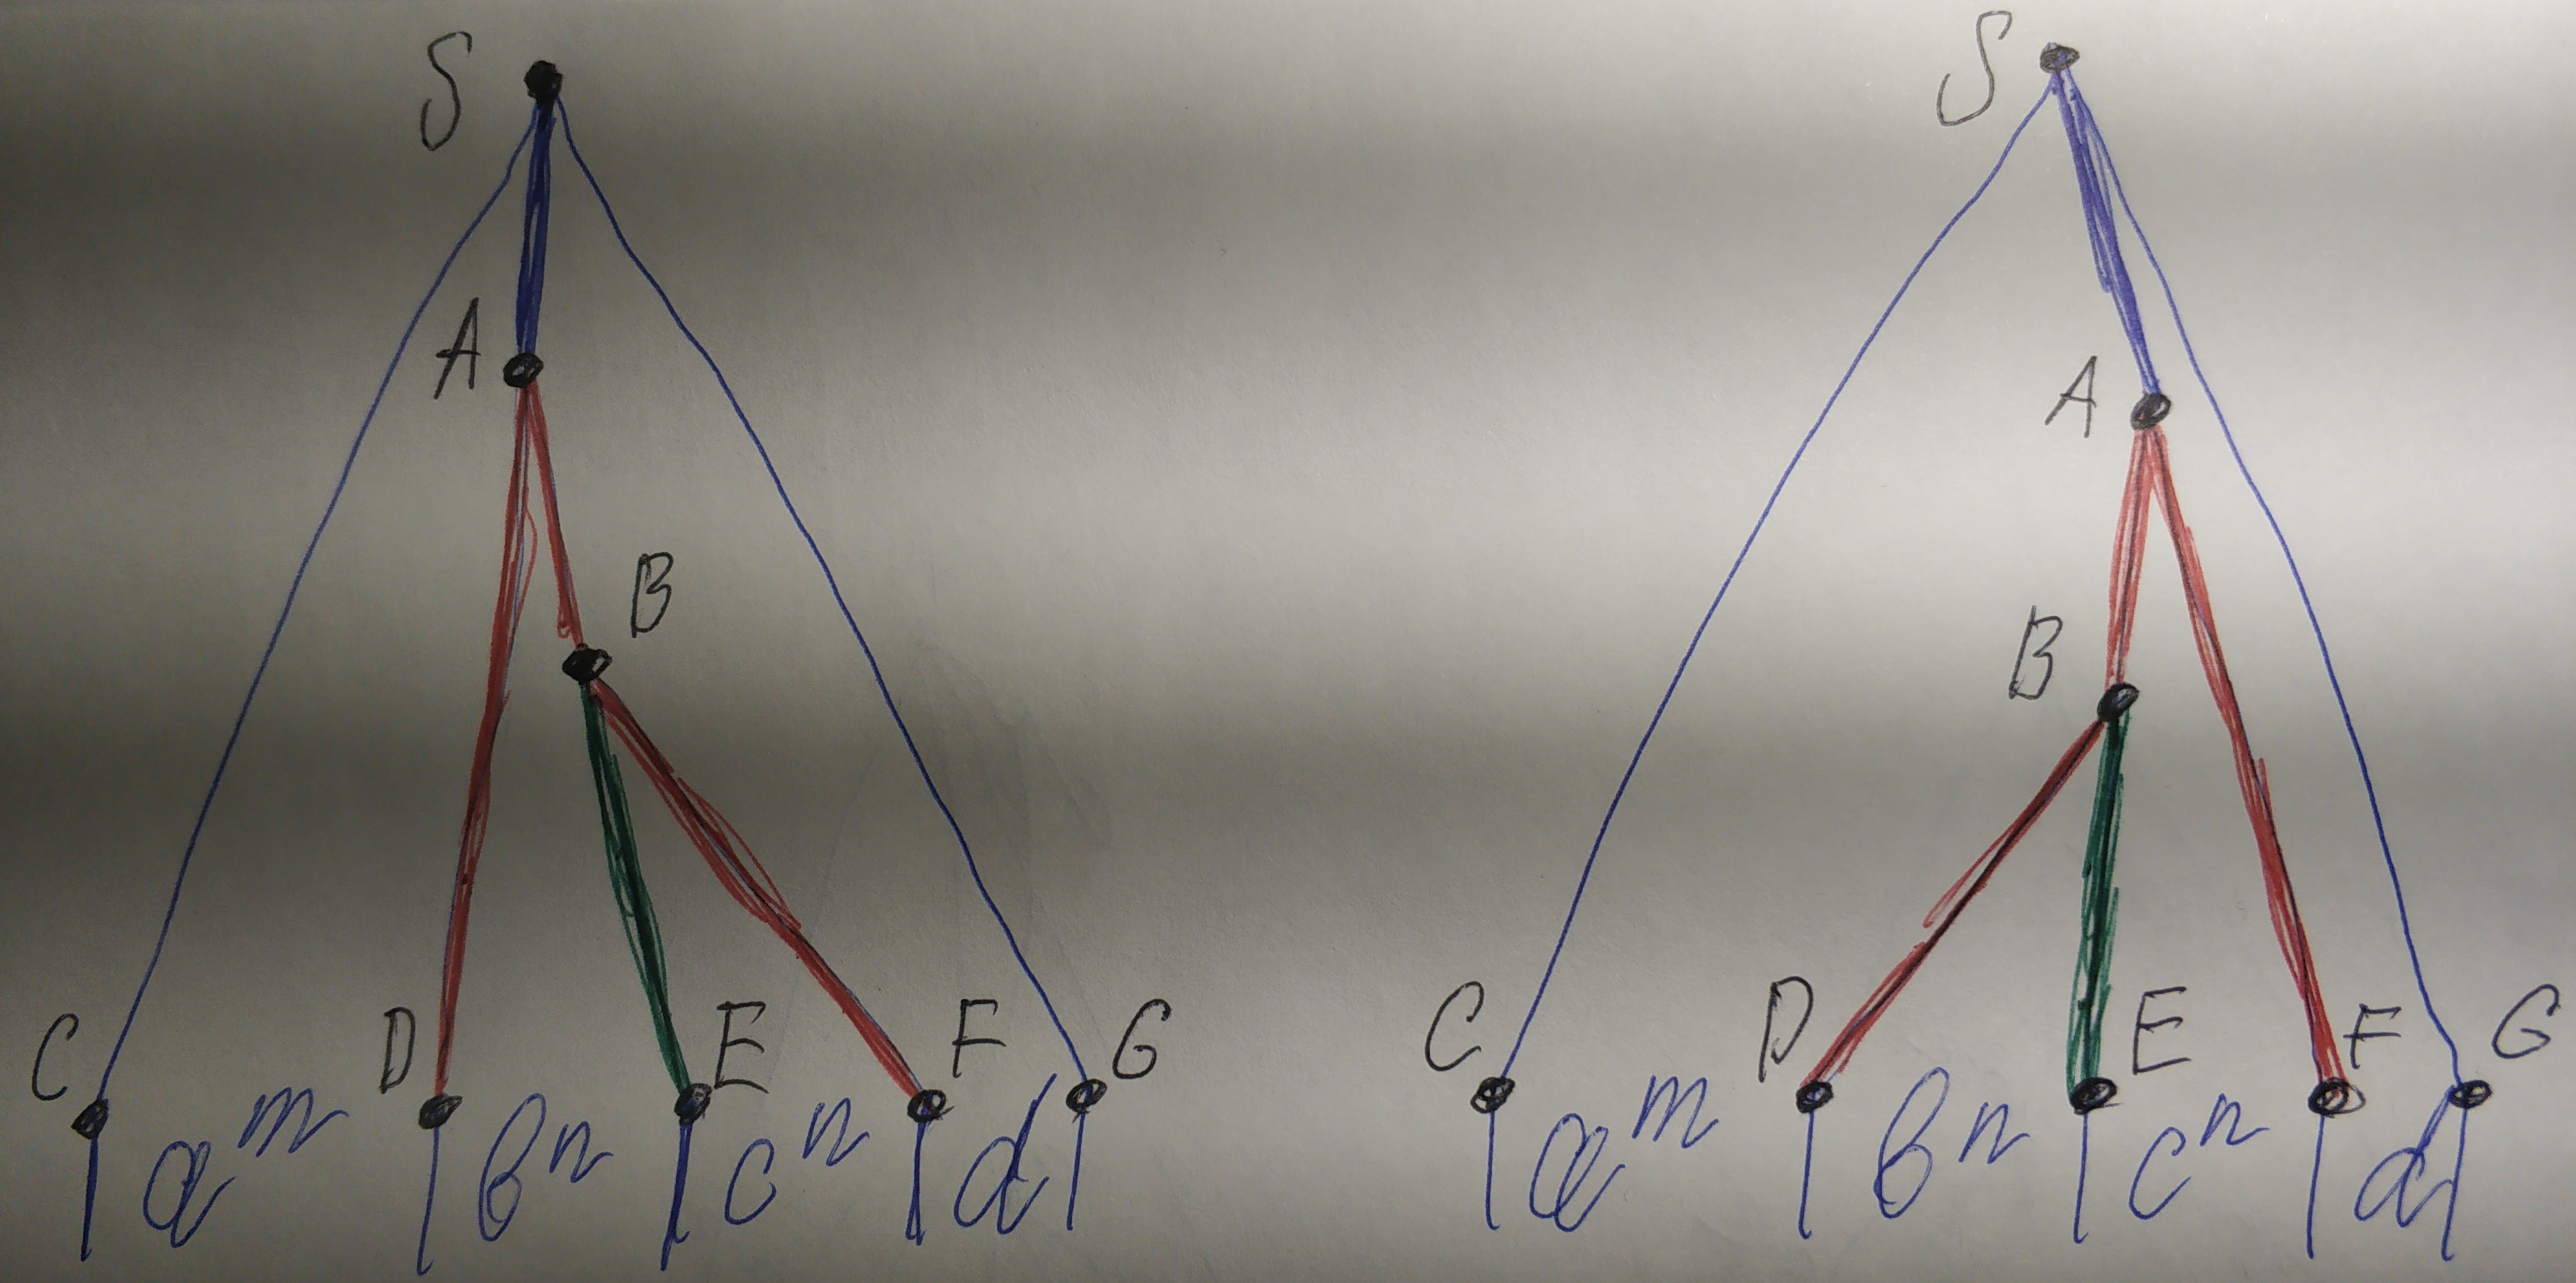
\includegraphics[height=7cm]{TI-HW-006-1.jpg}
        \end{figure}

        Несложно видеть, что на картинке красным отмечены части, которые не могут быть сколь угодно длинными, так как иначе можно найти на них два одинаковых нетерминала и получить слово, генерируемое грамматикой, но не из данного языка. Точнее:
        \begin{itemize}
            \item Ветви $AD$ на левой картинке и $AB$, $AD$ на правой должны быть короткими, так как иначе можно увеличиать один из блоков $b^n$ и $c^n$, не увеличивая другой; $d$ затронуто не будет.
            \item Ветви $AB$, $BF$ на левой картинке и $AF$ на правой должны быть короткими, так как иначе на них можно найти 3 (!) вершины с одним нетерминальным символом. Один из этих блоков точно не будет захватывать букву $d$, а значит будет расширять только блок $b^n$ или $c^n$. Имеем точно такое же противоречие.
        \end{itemize}
        Также зелёные части должны быть длинными, так как иначе у части $DABE$ на левой картинке и $DBE$ на правой будет короткий периметр, а тогда будет большая внутренность, тогда внутри можно выделить блок, который можно дублировать, т.е. можно увеличивать размер блока $b^n$, не меняя всё остальное. Тогда есть блок, который увеличивает блоки $b^n$ и $c^n$ на константу (если константы разные, то опять получаем противоречие, поэтому константа одна).

        % Также заметим, что если $SA$ на обеих картинках длинный, то будет три одинаковых нетерминальных символа, образующих два блока. Один блок точно не будет содержать буквы $d$, а тогда есть блок увеличивающий $a^m$. Если же он короткий, то у блока $a^m$ самого по себе есть такой же генератор.
        
        Заметим, что рассмотренные генераторы можно сделать ограниченными. Тогда для построения примера достачно взять $n$ и $m$ достаточно большими, что $m > n$ и $m-n$ делилось бы на все возможные размеры генераторов. Следовательно можно использовать генератор блоков $b^n$ и $c^n$, чтобы получить строку $a^m b^m c^m d$. Противоречие.
        
        Язык грамматикой не задаётся.
    \end{problem}

    \begin{problem}{6}
        Осмысленное описание грамматики выражений выглдит так:
        \begin{align*}
            E &\to 1 \mid x \mid (E) \mid S \mid P&
            St &\to 1 \mid x \mid P \mid (E)&
            S &\to St + St \mid S + St\\
            &&
            Pt &\to 1 \mid x \mid (E)&
            P &\to Pt \cdot Pt \mid P \cdot Pt
        \end{align*}
    \end{problem}

    \begin{problem}{7}
        Рассмотрим грамматику
        \begin{align*}
            S &\to TUVW&
            T &\to aT \mid a&
            U &\to bUc \mid bc&
            V &\to aVb \mid ab&
            W &\to cW \mid c.
        \end{align*}
        Несложно видеть, что $T$ порождает язык $aa^*$, $U$ --- $\{b^nc^n\}_{n > 0}$, $V$ --- $\{a^nb^n\}_{n > 0}$, $W$ --- $cc^*$. Следовательно, $S$ порождает язык $\{a^k b^n c^n a^m b^m c^l \mid k, l, m, n > 0\}$.

        \begin{lemma}
            $\sqrt{\{a^k b^n c^n a^m b^m c^l \mid k, l, m, n > 0\}} = \{a^n b^n c^n\}_{n > 0}$.
        \end{lemma}

        \begin{proof}
            Понятно, что для всякого слова $w \in \{a^n b^n c^n\}_{n > 0}$ слово
            \[ww \in \sqrt{\{a^k b^n c^n a^m b^m c^l \mid k, l, m, n > 0\}}.\]
            Покажем утверждение в обратную сторону: пусть дано слово
            \[ww \in \sqrt{\{a^k b^n c^n a^m b^m c^l \mid k, l, m, n > 0\}}.\]
            Имеем $ww = a^k b^n c^n a^m b^m c^l$, $k, l, m, n > 0$.
            
            Первое $w$ начинается на $a$, а второе заканчивается на $c$, значит это делают оба экземпляра. Значит первый экземпляр имеет последний элемент либо в блоке $c^n$, либо в блоке $c^l$. Значит он в любом случае начинается на $a^k b^n c$. По аналогии заканчивается на $a b^m c^l$. Значит первый экземпляр не может иметь последний элемент в блоке $c^l$, а поэтому содержит его в блоке $c^n$; аналогично второй экземпляр содержит первый элемент в блоке $a^m$. Значит граница между экземплярами --- граница между блоками $c^n$ и $a^m$. Таким образом
            \[w = a^k b^n c^n = a^m b^m c^l.\]
            Т.е. $k = m = n = l > 0$. Таким образом $w \in \{a^n b^n c^n\}_{n > 0}$.
        \end{proof}

        Как мы знаем (по лемме о накачке) $\{a^n b^n c^n\}_{n > 0}$ не порождается грамматикой. Таким образом мы построили язык, порождаемый грамматикой, чей корень не задаётся грамматикой.
    \end{problem}

    \begin{problem}{8}
        \newcommand{\Permutations}{\mathrm{Permutations}}
        \textbf{Небольшое уточнение формулировки задачи.} Пусть $L$ --- регулярный язык. Верно ли, что язык, состоящий из всевозможных перестановок символов в словах из $L$, задаётся грамматикой? Будем обозначать такой язык $\Permutations(L)$.

        Рассмотрим случаи размера алфавита.
        \begin{enumerate}
            \item $|\Sigma| = 1$. Очевидно, что перестановки символов в слове ничего не делают, поэтому просто грамматизации автомата хватит, чтобы породить искомый язык грамматикой.

            \item $|\Sigma| = 3$; $\Sigma = \{a; b; c\}$. Рассмотрим регулярный язык $L = (abc)^*$ (регулярный он потому, что мы только что задали его регулярным выражением). Тогда
                \[L' := \Permutations(L) = \{w \in \Sigma^* \mid |w|_a = |w|_b = |w|_c\}.\]
                Т.е. $\{a^n b^n c^n\}_{n \geqslant 0} \subseteq L'$. Предположим, что $L'$ задаётся грамматикой $(\Sigma, N, R, S)$.
                
                Посмотрим дерево разбора какой-нибудь строки $a^n b^n c^n$. Рассмотрим границу между блоками $a^n$ и $b^n$, и будем подниматься по ней вверх по дереву. Сначала мы будем идти между соседними ветями деревьев, а потом вонзимся в какую-то вершину (нетерминальный символ) дерева и будем рассекать соответствующую ветвь дерева до самого дерева.
                \begin{figure}[H]
                    \centering
                    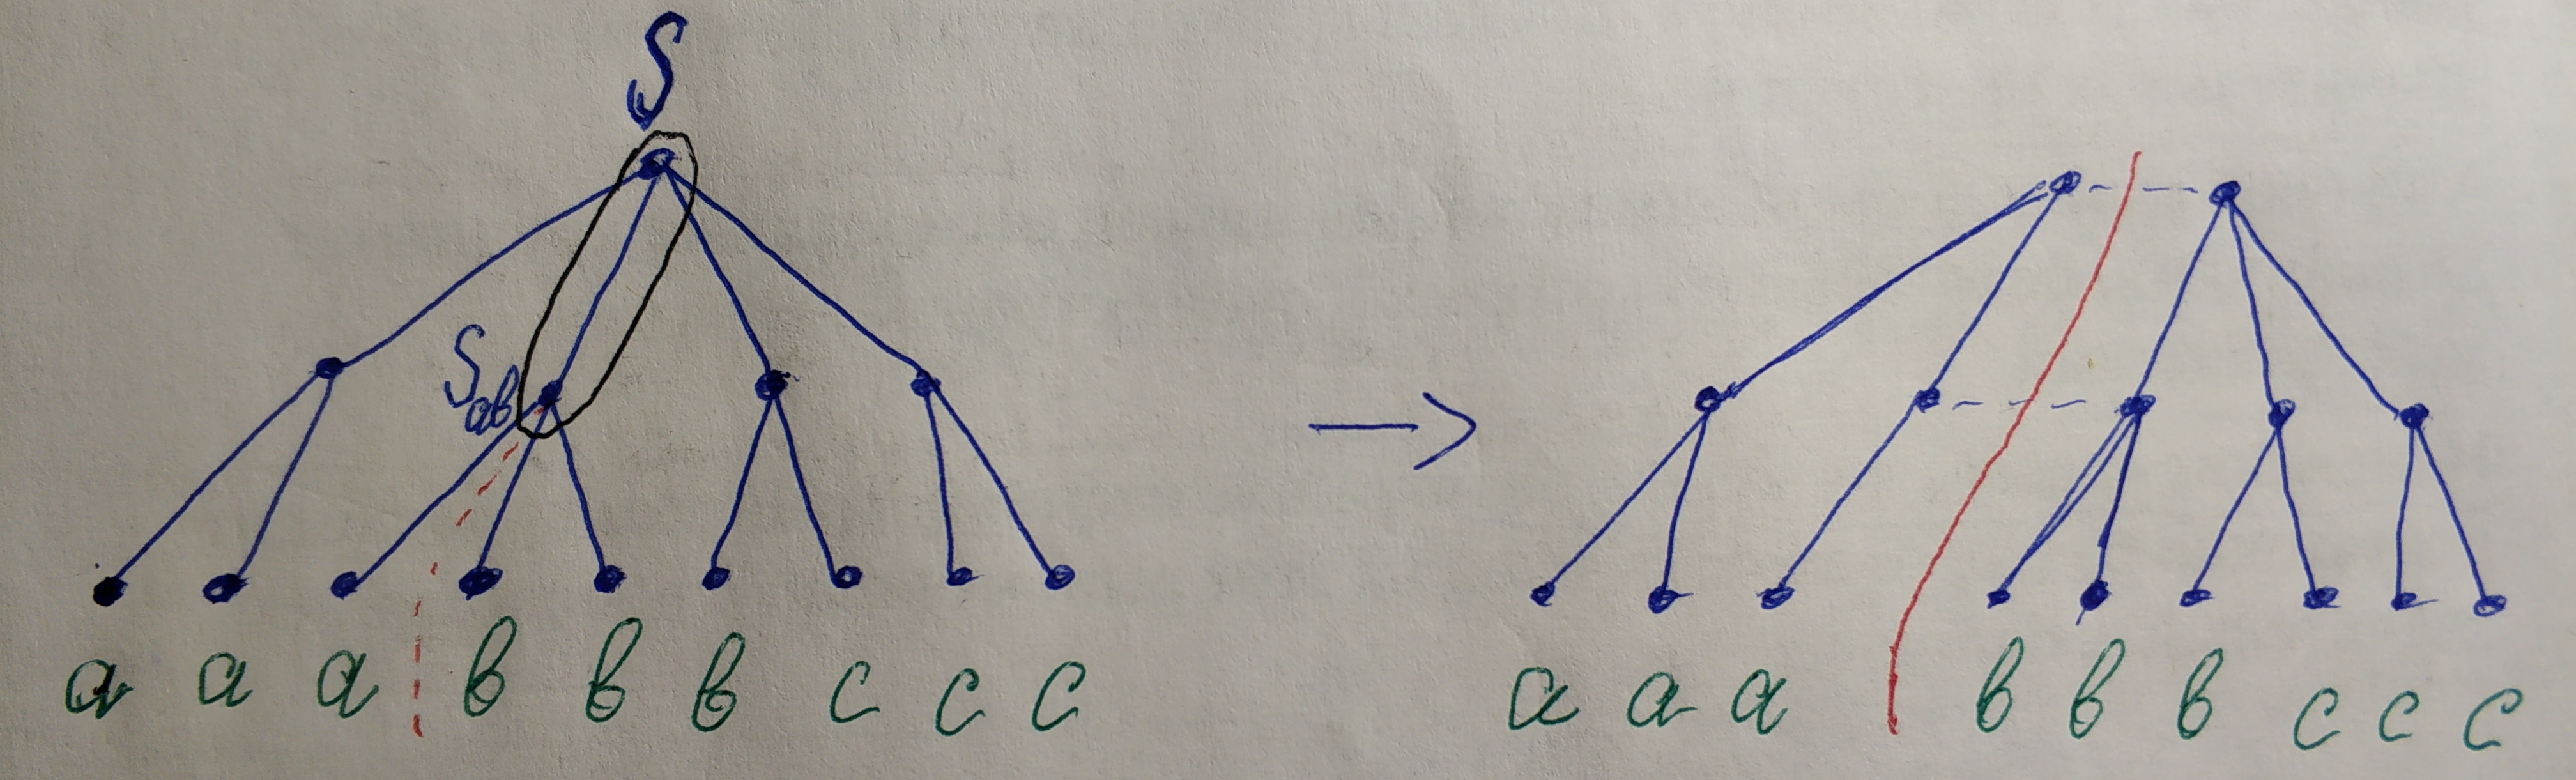
\includegraphics[height=5cm]{TI-HW-006-2.jpg}
                \end{figure}
                Назовём первую разрезаемую вершину $S_{ab}$ (т.е. мы таким способом разрезали ветвь (путь) $S \to S_{ab}$). Аналогично для разделителя блоков $b^n$ и $c^n$ определим первую разрезаемую вершину $S_{bc}$. Также назовём самую нижнюю общую ввершину ветвей $S \to S_{ab}$ и $S \to S_{bc}$ за $S'$.
                
                Если количество вершин в пути $S' \to S_{ab}$, включая $S_{ab}$, но исключая $S'$, хотя бы $|N| + 1$, то в этом пути есть две вершины с одинаковыми нетерминальными символами, а значит (как в лемме о накачке) промежуток между ними можно дублировать сколь угодно много раз. Поскольку все рассматриваемые вершины строго левее ветви $S \to S_{bc}$, то блок $c^n$ затронут не будет. Значит мы получим новую строку, где количество $a$ и $b$ изменилось (так как данный блок находится на ветви $S' \to S_{ab}$, и поэтому захватывает и кусок из блока $a^n$, и кусок блока $b^n$), а количество $c$ не изменилось, что противоречит с определением рассмотренной грамматики. Значит пути $S' \to S_{ab}$ и $S' \to S_{bc}$ ограничены по длине.

                Заметим, что все символы $b$ являются листьями на ветвях, растущих либо с вершины ветви $S' \to S_{ab}$ вправо, либо с вершин ветви $S' \to S_{bc}$ влево, либо из $S'$ между ветвями $S' \to S_{ab}$ и $S' \to S_{bc}$. Мысленно отрубим всё остальное. Получим дерево (не разбора) блока $b^n$ с корнем $S'$.
                
                Пусть $s$ и $p$ --- максимальные количества терминальных и нетерминальных символов в подстановочных строках правил соответственно. Тогда в любом дереве глубины не более $d$ (уровень корня --- $1$) будет не более $\frac{p^d - 1}{p - 1}$. Вернёмся к нашему огрызочному дереву. На пути $S_{ab} \to S' \to S_{bc}$ суммарно не более $2|N| + 1$ вершин. Значит, если мы оторвём все эти вершины, то получим не более $p(2|N| + 1)$ деревьев. Если ни в каком из этих деревьев нет двух вершин, одна над другой, с одинаковыми нетерминальными символами, то всякая ветвь (путь сверху вниз) в них имеет длину (в вершинах) не более $|N|$, т.е. всякое из получившехся деревцев имеет глубину не более $|N|$, т.е. каждое из них имеет размер не более $\frac{p^{|N|} - 1}{p - 1}$, т.е. всего вершин в огрызочном дереве не более $p(2|N| + 1)\frac{p^{|N|} - 1}{p - 1} + (2|N| + 1)$, а значит огрызочное дерево порождает строку длины не более
                \[s\left(p(2|N| + 1)\frac{p^{|N|} - 1}{p - 1} + (2|N| + 1)\right).\]
                При этом в блоке $b^n$ ровно $n$ символов и мы не ставили никаких ограничений на $n$ (т.е. могли взять строку для сколь угодно большого $n$). Поэтому если $n$ будет больше этой величины, то будет ветвь между двумя одинаковыми нетерминальными символами, находящаяся строго между ветвями $S' \to S_{ab}$ и $S' \to S_{bc}$. Тогда как лемме о накачке можно дублировать эту ветвь сколь угодно много раз. И поскольку эта ветвь находится строго между описанными ранее ветвями, то она затрагивает только два куска в блоке $b^n$, а значит мы получим строку с новым количеством символов $b$ и неизменными количествами символов $a$ и $c$. Это опять противоречит определению грамматики.

                Итого, нет грамматики, порождающей $L'$.

            \item $|\Sigma| \geqslant 3$. Несложно видеть, что всякий ДКА на трёхсимвольном алфавите --- это НКА на большем алфавите. Как мы показали, есть регулярный язык на трёхсимвольном алфавите, чей перестановочный язык не порождается грамматикой, а значит, рассматривая его как регулярный язык над большим алфавитом, получаем, что он всё ещё не порождается грамматикой. Поэтому ответ всё тот же: нет не всегда.

            \item $|\Sigma| = 2$; $\Sigma = \{a; b\}$. Как мы знаем, $L$ порождается регулярным выражением. Но для построения $L' := \Permutations(L)$ важно не столь какие слова содержатся в $L$, сколь какие пары $(|w|_a; |w|_b)$ достигаются хоть одним словом $w \in L$, так как задача будет состоять в том, чтобы расположить ровно $|w|_a$ символов $a$ и ровно $|w|_b$ символов $b$ в абсолютно любом порядке. Поэтому сделаем следующий трюк.
            
                Договоримся во всякой грамматике обозначать язык, порождаемый нетерминальным символом $A$, за $L(A)$.
            
                \begin{definition}
                    Для всякого слова $w$ обозначим вектор $(|w|_a; |w|_b)$ за $C(w)$ или $\overline{w}$ и будем называть его \emph{вектором (вхождений) слова $w$}. Также для всякого языка $L$ обозначим
                    \[C(L) := \{C(w)\}_{w \in L}.\]
                    $C(L)$ будем называть \emph{множеством векторов (вхождений) языка $L$}.
                    
                    Для всякого множества $V$ векторов из $\ZZ^2$ (или же $(\NN \cup \{0\})^2$) обозначим
                    \[L(V) := \{w \in \Sigma^* \mid \overline{w} \in V\}.\]

                    Определим также операции на $\mathcal{P}(\ZZ^2)$.
                    \begin{itemize}
                        \item $V + U := \{v + u \mid v \in V \wedge u \in U\}$.
                        \item $V \cup U$ --- обычное объединение множеств.
                        \item $nV := \underbrace{V + \dots + V}_{n}$. $0V := \{(0; 0)\}$.
                        \item $V^* := \bigcup_{n=0}^\infty nV$.
                    \end{itemize}

                    Назовём \emph{регулярными выражениями над множествами (из $\ZZ^2$)} выражения построенные по следующим рекуррентным правилам:
                    \begin{itemize}
                        \item $\varnothing$ --- регулярное выражение.
                        \item $\{(1; 0)\}$ и $\{(0; 1)\}$ --- регулярные выржения.
                        \item $(t + s)$, $(t \cup s)$ и $t^*$, где $t$ и $s$ суть регулярные выражения, --- регулярные выражения.
                    \end{itemize}
                    Для всякого регулярного выражения $t$ над множествами обозначим $S(t)$ значение выражения $t$, а за $L(t)$ значение $L(S(t))$. Формально, рекуррентно определим $S$ правилами
                    \begin{itemize}
                        \item $S(\varnothing) := \varnothing$,
                        \item $S(\{(1; 0)\}) := \{(1; 0)\}$, $S(\{(1; 0)\}) = \{(1; 0)\}$,
                        \item $S((t + s)) = S(t) + S(s)$,
                        \item $S((t \cup s)) = S(t) \cup S(s)$,
                        \item $S(t^*) = S(t)^*$.
                    \end{itemize}

                    Также сопоставим обычным регулярным выражениям регулярные выражения над множествами (и наоборот) заменой $\varnothing$ на $\varnothing$, $a$ --- на $\{(1; 0)\}$, $b$ --- на $\{(0; 1)\}$, $\cdot$ (конкатенация) --- на $+$, $\mid$ --- на $\cup$, ${}^*$ --- на ${}^*$. Т.е. формально,
                    \begin{itemize}
                        \item $\varnothing$ соответствует $\varnothing$ и наоборот,
                        \item $a$ соответствует $\{(1; 0)\}$ и наоборот,
                        \item $b$ соответствует $\{(0; 1)\}$ и наоборот,
                        \item если $\tau$ соответствует $T$, а $\sigma$ --- $S$, то $(\tau\sigma)$ соответствует $(T + S)$ и наоборот,
                        \item если $\tau$ соответствует $T$, а $\sigma$ --- $S$, то $(\tau|\sigma)$ соответствует $(T \cup S)$ и наоборот,
                        \item если $\tau$ соответствует $T$, то $\tau^*$ соответствует $T^*$ и наоборот. 
                    \end{itemize}
                    Соответствующие друг другу выражения так и назовём \emph{соответствующими}.
                \end{definition}

                \begin{lemma}\ 
                    \begin{enumerate}
                        \item Пусть дано семейство языков $\{M_i\}_{i \in I}$. Тогда
                            \[C\left(\bigcup_{i \in I} M_i\right) = \bigcup_{i \in I} C(M_i).\]
                        \item Пусть дано семейство языков $\{M_i\}_{i \in I}$. Тогда
                            \[C\left(\bigcap_{i \in I} M_i\right) \subseteq \bigcap_{i \in I} C(M_i).\]
                        \item Пусть даны языки $M$ и $N$, что $M \subseteq N$. Тогда $C(M) \subseteq C(N)$.
                        \item Пусть дано семейство множеств векторов $\{V_i\}_{i \in I}$. Тогда
                            \[L\left(\bigcup_{i \in I} V_i\right) = \bigcup_{i \in I} L(V_i).\]
                        \item Пусть дано семейство множеств векторов $\{V_i\}_{i \in I}$. Тогда
                            \[L\left(\bigcap_{i \in I} V_i\right) = \bigcap_{i \in I} L(V_i).\]
                        \item Пусть даны множества векторов $V$ и $U$, что $V \subseteq U$. Тогда $L(V) \subseteq L(U)$.
                        \item Для всякого языка $M$ верно $L(C(M)) \supseteq M$. Равенство достигается тогда и только тогда, когда $M$ замкнуто относительно операции взятия всевозможных перестановок символов слов.
                        \item Для всякого множества векторов $V$ верно $C(L(V)) = V$.
                        \item Для всяких языков $M$ и $N$ верно $C(MN) = C(M) + C(N)$.
                        \item Для всякого языка $M$ и $n \in \NN \cup \{0\}$ верно $C(M^n) = nC(M)$.
                        \item Для всякого языка $M$ верно $C(M^*) = C(M)^*$.
                        \item $V + U = U + V$.
                        \item $nV + mV = (n+m)V$.
                        \item $(V \cup U) + W = V + W \cup U + W$.
                        \item $n(V \cup U) = \bigcup_{k = 0}^n kV + (n-k)U$ (почти бином Ньютона).
                        \item $(V \cup U)^* = V^* + U^*$.
                        \item $nV^* = V^*$ при $n > 0$. (По определению $0V^* = \{(0; 0)\}$.)
                        \item $(V + U^*)^* = \{(0; 0)\} \cup V + V^* + U^* = \{(0; 0)\} \cup V + (V \cup U)^*$.
                    \end{enumerate}
                \end{lemma}

                \begin{proof}\ 
                    \begin{enumerate}
                        \item Для всякого вектора $p \in C\left(\bigcup_{i \in I} M_i\right)$ есть вектор $w \in \bigcup_{i \in I} M_i$ с этим вектором. При этом $w$ лежит в некотором $M_j$, а тогда $p \in C(M_j)$. Следовательно, $p \in \bigcup_{i \in I} C(M_i)$. Таким образом
                            \[C\left(\bigcup_{i \in I} M_i\right) \subseteq \bigcup_{i \in I} C(M_i).\]

                            Всякий вектор $p \in \bigcup_{i \in I} C(M_i)$ лежит в некотором $C(M_j)$. Тогда есть слово $w \in M_j$ с этим вектором. Тогда $w \in \bigcup_{i \in I} M_i$. Следовательно, $p \in C\left(\bigcup_{i \in I} M_i\right)$. Таким образом
                            \[C\left(\bigcup_{i \in I} M_i\right) \supseteq \bigcup_{i \in I} C(M_i).\]
                        
                        \item Для всякого вектора $p \in C\left(\bigcap_{i \in I} M_i\right)$ есть вектор $w \in \bigcap_{i \in I} M_i$ с этим вектором. Значит $w$ лежит во всяком $M_j$. Тогда $p$ лежит во всяком $C(M_j)$. Значит
                            \[C\left(\bigcap_{i \in I} M_i\right) \subseteq \bigcap_{i \in I} C(M_i).\]

                        \item $C(N) = C(N \setminus M) \cup C(M) \supseteq C(M)$.

                        \item Для всякого $w \in L\left(\bigcup_{i \in I} V_i\right)$ верно $\overline{w} \in \bigcup_{i \in I} V_i$, значит $\overline{w}$ лежит в каком-то $V_j$. Следовательно $w \in L(V_j)$, а тогда $w \in \bigcup_{i \in I} L(V_i)$. Таким образом
                            \[L\left(\bigcup_{i \in I} V_i\right) \subseteq \bigcup_{i \in I} L(V_i).\]

                            Всякий $w \in \bigcup_{i \in I} L(V_i)$ лежит в некотором $L(V_j)$. Тогда $\overline{w} \in V_j$, т.е. $\overline{w} \in \bigcup_{i \in I} V_i$. Следовательно, $w \in L\left(\bigcup_{i \in I} V_i\right)$. Таким образом
                            \[L\left(\bigcup_{i \in I} V_i\right) \supseteq \bigcup_{i \in I} L(V_i).\]
                            
                        \item Для всякого $w \in L\left(\bigcap_{i \in I} V_i\right)$ верно $\overline{w} \in \bigcap_{i \in I} V_i$, значит $\overline{w}$ лежит во всех $V_j$. Следовательно $w$ лежит во всех $L(V_j)$, а тогда $w \in \bigcap_{i \in I} L(V_i)$. Таким образом
                            \[L\left(\bigcap_{i \in I} V_i\right) \subseteq \bigcap_{i \in I} L(V_i).\]

                            Всякий $w \in \bigcap_{i \in I} L(V_i)$ лежит во всех $L(V_j)$. Тогда $\overline{w}$ лежит во всех $V_j$, т.е. $\overline{w} \in \bigcap_{i \in I} V_i$. Следовательно, $w \in L\left(\bigcap_{i \in I} V_i\right)$. Таким образом
                            \[L\left(\bigcap_{i \in I} V_i\right) \supseteq \bigcap_{i \in I} L(V_i).\]

                        \item $L(U) = L(U \setminus V) \cup L(V) \supseteq L(V)$.
                        
                        \item Если $w \in M$, то $\overline{w} \in C(M)$, а тогда $w \in L(C(M))$. Таким образом $M \subseteq L(C(M))$. При этом если $M \neq L(C(M))$, то есть $w \in L(C(M)) \setminus M$, но тогда $\overline{w} \in C(M)$, а значит есть $v \in M$, что $\overline{v} = \overline{w}$. Тогда $w$ --- перестановка символов $v$, которая не лежит в $M$, т.е. $M$ не замкнуто относительно операции взятия всевозможных перестановок символов слов. Если $M$ не замкнуто относительно данной операции, то есть $v \in M$, что некоторая перестановка его символов $w$ не лежит в $M$. Но тогда $\overline{w} = \overline{v} \in C(M)$, а значит $w \in L(C(M))$.

                        \item Для всякого $p \in V$ есть $w \in L(V)$ с данным вектором, а значит $p \in C(L(V))$. При этом если $p \in C(L(V))$, то есть $w \in L(V)$ с данным вектором, а значит $p \in V$.

                        \item Для всякого $p \in C(MN)$ есть $w \in MN$ с этим вектором. Тогда $w = vu$ для некоторых $v \in M$, $u \in N$. Следовательно $p = \overline{w} = \overline{v} + \overline{u} \in C(M) + C(N)$.

                            При этом для всякого $p \in C(M) + C(N)$ есть $q \in C(M)$ и $r \in C(N)$, что $p = q + r$. Следовательно есть $v \in M$ и $u \in N$, что $\overline{v} = q$, $\overline{u} = r$. Значит $vu \in MN$, а тогда $p = q + r = \overline{v} + \overline{u} = \overline{vu} \in C(MN)$.
                        
                        \item Если $n > 0$, то утверждение выходит из прошлого пункта. Если $n = 0$, то $C(M^n) = C(\{\varepsilon\}) = \{(0; 0)\} = nC(M)$.
                        
                        \item
                            \[C(M^*) = C\left(\bigcup_{n=0}^\infty M^n\right) = \bigcup_{n=0}^\infty C(M^n) = \bigcup_{n=0}^\infty nC(M) = C(M)^*.\]
                        \item Коммутативность суммы Минковского наследуется от изначального оператора.
                        \item
                            \[
                                nV + mV
                                = \underbrace{V + \dots + V}_n + \underbrace{V + \dots + V}_m
                                = \underbrace{V + \dots + V}_{n+m}
                                = (n+m)V.
                            \]
                        \item
                            \begin{align*}
                                (V \cup U) + W
                                &= \{v + w \mid v \in V \cup U \wedge w \in W\}\\
                                &= \{v + w \mid v \in V \wedge w \in W\} \cup \{v + w \mid v \in U \wedge w \in W\}\\
                                &= V + W \cup U + W.
                            \end{align*}
                        \item Несложно показать это утверждение по индукции с помощью следующего шага.
                            \begin{align*}
                                (n+1)(V \cup U)
                                &= n(V \cup U) + (V \cup U)\\
                                &= (nV \;\; \cup \;\; (n-1)V + U \;\; \cup \;\; \dots \;\; \cup \;\; V + (n-1)U \;\; \cup \;\; nU) + (V \cup U)\\
                                &= (nV + (V \cup U)) \;\; \cup \;\; ((n-1)V + U + (V \cup U)) \;\; \cup \;\; \dots\\
                                &\qquad \cup \;\; (V + (n-1)U + (V \cup U)) \;\; \cup \;\; (nU + (V \cup U))\\
                                &= ((n+1)V \;\; \cup \;\; nV + U)) \;\; \cup \;\; (nV + U \;\; \cup \;\; (n-1)V + 2U) \;\; \cup \;\; \dots\\
                                &\qquad \cup \;\; (2V + (n-1)U \;\; \cup \;\; V + nU) \;\; \cup \;\; (nU + V \;\; \cup \;\; (n+1)U)\\
                                &= (n+1)V \;\; \cup \;\; nV + U \;\; \cup \;\; \dots \;\; \cup \;\; V + nU \;\; \cup \;\; (n+1)U
                            \end{align*}
                        \item
                            \[
                                (V \cup U)^*
                                = \bigcup_{n=0}^\infty n(V \cup U)
                                = \bigcup_{k,l=0}^\infty kV + lU
                                = \left(\bigcup_{k=0}^\infty kV\right) + \left(\bigcup_{l=0}^\infty lU\right).
                            \]
                        \item
                            \begin{align*}
                                nV^*
                                &= n \bigcup_{m=0}^\infty mV&
                                &= \bigcup_{m_1 = 0}^\infty m_1 V + \dots + \bigcup_{m_n = 0}^\infty m_n V\\
                                &= \bigcup_{m_1, \dots, m_n = 0}^\infty (m_1 + \dots + m_n)V&
                                &= \bigcup_{m = 0}^\infty \; \bigcup_{m_1 + \dots + m_n = m} mV\\
                                &= \bigcup_{m = 0}^\infty mV&
                                &= V^*
                            \end{align*}
                        \item
                            \begin{align*}
                                (V + U^*)^*
                                &= \bigcup_{n=0}^\infty n(V + U^*)&
                                &= \bigcup_{n=0}^\infty nV + nU^*\\
                                &= \{(0; 0)\} \cup \bigcup_{n=1}^\infty nV + U^*&
                                &= \{(0; 0)\} \cup V + V^* + U^*
                            \end{align*}
                    \end{enumerate}
                \end{proof}

                \begin{lemma}\ 
                    \begin{enumerate}
                        \item Если $\tau$ и $t$ --- соответствующие друг другу регулярное выражение и регулярное выражение для множеств, то $C(L(\tau)) = S(t)$.
                        \item Для всякого регулярного языка $L$ множество $C(L)$ задаётся некоторым регулярным выражением на множествах $t$.
                        \item Для всякого регулярного выражения на множествах $t$ есть регулярный язык $L$, что $C(L) = S(t)$.
                        \item TFAE
                            \begin{itemize}
                                \item (Изначальная задача.) Для всякого регулярного языка $L$ язык $L(C(L))$ грамматизируется.
                                \item Для всякого регулярного выражения на множествах $t$ язык $L(t)$ грамматизируется.
                            \end{itemize}
                        \item \label{RE-normal-form} Всякое регулярное выражение над множествами с непустым значением упрощается без изменения значения до выражения вида
                            \[
                                (E_1) \cup \dots \cup (E_n),
                                \qquad \text{ где } \qquad
                                E_i = \{v_i\} + \{u_{i, 1}\}^* + \dots + \{u_{i, k_i}\}^*,
                            \]
                            где $v_i$ и $u_{i, j}$ --- некоторые вектора из $(\NN \cup \{0\})^2$, $n \geqslant 1$, $k_i \geqslant 0$.
                        \item Всякое выражение как в \ref{RE-normal-form} несильно модифицируется без изменения значения в регулярное выражение.
                        \item TFAE
                            \begin{itemize}
                                \item Для всякого регулярного выражения на множествах $t$ язык $L(t)$ грамматизируется.
                                \item Для всякого выражения $t$ как в \ref{RE-normal-form} язык $L(t)$ грамматизируется.
                            \end{itemize}
                    \end{enumerate}
                \end{lemma}

                \begin{proof}
                    \begin{enumerate}
                        \item Докажем это по индукции по $\tau$.

                            \begin{itemize}
                                \item Если $\tau = \varnothing$, то $t = \varnothing$. Тогда $C(L(\tau)) = C(\varnothing) = \varnothing = S(t)$.
                                \item Если $\tau = a$, то $t = \{(1; 0)\}$. Тогда $C(L(\tau)) = C(\{a\}) = \{(1; 0)\} = S(t)$.
                                \item Если $\tau = b$, то $t = \{(0; 1)\}$. Тогда $C(L(\tau)) = C(\{b\}) = \{(0; 1)\} = S(t)$.
                                \item Если $\tau = (\sigma\rho)$, то $\sigma$ и $\rho$ соответствуют $s$ и $r$, и $t = (s + r)$. А значит $C(L(\tau)) = C(L(\sigma) L(\rho)) = C(L(\sigma)) + C(L(\rho)) = S(s) + S(r) = S(t)$.
                                \item Если $\tau = (\sigma|\rho)$, то $\sigma$ и $\rho$ соответствуют $s$ и $r$, и $t = (s \cup r)$. А значит $C(L(\tau)) = C(L(\sigma) \cup L(\rho)) = C(L(\sigma)) \cup C(L(\rho)) = S(s) \cup S(r) = S(t)$.
                                \item Если $\tau = \sigma^*$, то $\sigma$ соответствует $s$, и $t = s^*$. А значит $C(L(\tau)) = C(L(\sigma)^*) = C(L(\sigma))^* = S(s) + S(r) = S(t)$.
                            \end{itemize}
                        \item Всякий регулярный язык $L$ задаётся регулярным выражением $\tau$. Пусть $t$ --- регулярное выражение на множествах, ему соответствующее. Тогда $C(L) = C(L(\tau)) = S(t)$.
                        \item Для всякого регулярного выражения на множествах $t$ есть ему соответствующее выражение $\tau$, а значит $L := L(\tau)$ --- регулярный язык. Тогда $C(L) = C(L(\tau)) = S(t)$.
                        \item Если второе утверждение верно, то тогда для всякого регулярного языка $L$ есть регулярное выражение на множествах $t$, что $C(L) = S(t)$. Тогда $L(C(L)) = L(S(t)) = L(t)$ грамматизируется. Это значит, что верно первое.

                            Если верно первое, то для всякого регулярного выражения на множествах $t$ есть регулярный язык, что $S(t) = C(L)$. Тогда язык $L(t) = L(S(t)) = L(C(L))$ грамматизируется.
                        \item Так как нет лучше метода, чем (полная) индукция, то будем доказывать, что всякое такое выражение упрощается до указанного вида, индукцией по размеру выражения (на деле индукцией по структуре выражения). (Полная индукция --- это индукция, где шаг использует все предыдущие утверждения. Поэтому у неё нет базы!)
                            
                            Пусть дано выражение $p$.
                            \begin{itemize}
                                \item Если $p = \varnothing$, то значение $\varnothing$ пусто.
                                \item Если $p = \{(1; 0)\}$ или $p = \{(0; 1)\}$, то оно уже имеет подобающий вид. Т.е. $p = E_1$, где $E_1 = \{v_1\}$, $v_1 = (1; 0)$ (или $(0; 1)$), т.е. $n = 1$, $k_1 = 0$.
                                \item Если $p = q \cup r$, то по предположению индукции $q$ и $r$ можно заменить на $q'$ и $r'$, имеющие то же значение, или их значения пусты. Если значения $q$ и $r$ пусты, то пусто и значение $p$. Если пусто только $q$, то $r'$ будет значить то же, что и $p$, и иметь подобающий вид; аналогично если пусто только $r$. Иначе $p' = q' \cup r'$ будет значить то же, что и $p$, и иметь подобающий вид.
                                \item Если $p = q + r$, то по предположению индукции $q$ и $r$ можно заменить на $q'$ и $r'$, имеющие то же значение, или их значения пусты. Если пусто хотя бы одно из значений $q$ и $r$, то пусто и $q$. Поэтому рассмотрим случай, когда значения $q$ и $r$ непусты. Тогда
                                    \[
                                        q' = (E_1) \cup \dots \cup (E_n),
                                        \qquad
                                        r' = (F_1) \cup \dots \cup (F_m).
                                    \]
                                    Понятно, что в смысле выражений
                                    \[
                                        p
                                        = q + r
                                        = q' + r'
                                        = \bigcup_{i=1}^n E_i + \bigcup_{j=1}^m F_j
                                        = \bigcup_{\substack{i=1,\dots,n\\ j=1,\dots,m}} E_i + F_j.
                                    \]
                                    По определению
                                    \[
                                        E_i = \{v_i\} + \{u_{i, 1}\}^* + \dots + \{u_{i, k_i}\}^*,
                                        \qquad
                                        F_j = \{x_j\} + \{y_{j, 1}\}^* + \dots + \{y_{j, l_j}\}^*.
                                    \]
                                    Понятно, что в смысле выражений
                                    \begin{align*}
                                        E_i + F_j
                                        &= \left(\{v_i\} + \sum_{t=1}^{k_i} \{u_{i, t}\}^*\right) + \left(\{x_j\} + \sum_{s=1}^{l_j} \{y_{j, s}\}^*\right)\\
                                        &= \{v_i + x_j\} + \sum_{t=1}^{k_i} \{u_{i, t}\}^* + \sum_{s=1}^{l_j} \{y_{j, s}\}^*.
                                    \end{align*}
                                    Тогда последнее выражение (в расписанном виде, без знаков суммы) можно обозначить за $G_{i, j}$. Тогда
                                    \[p' := G_{1, 1} + \dots + G_{n, 1} + G_{1, 2} + \dots + G_{n, m}\]
                                    имеет то же значение, что и $p$, и имеет подобающий вид.
                                \item Если $p = q^*$, то по предположению индукции $q$ можно заменить на $q'$, имеющее то же значение, или его значение пусто. Если значение $q$ пусто, то значение $p$ --- $\{(0; 0)\}$, что представляется в подобающем виде так же, как $\{(1; 0)\}$ и $\{(0; 1)\}$. Поэтому будем считать, что значение $q$ непусто. Тогда
                                    \[q' = (E_1) \cup \dots \cup (E_n).\]
                                    Тогда в смысле варажений
                                    \[p = q^* = (q')^* = \left(\bigcup_{i=1}^n E_i\right)^* = \sum_{i=1}^n E_i^*.\]
                                    По определению
                                    \[E_i = \{v_i\} + \{u_{i, 1}\}^* + \dots + \{u_{i, k_i}\}^*.\]
                                    Тогда в смысле выражений
                                    \[E_i = \{v_i\} + \sum_{j=1}^{k_i} \{u_{i, j}\}^* = \{v_i\} + (\{u_{i, j}\}_{j=1}^{k_i})^*,\]
                                    а значит
                                    \[E_i^* = \{(0; 0)\} \cup \{v_i\} + (\{v_i\} \cup \{u_{i, j}\}_{j=1}^{k_i})^*,\]
                                    т.е.
                                    \begin{align*}
                                        p
                                        &= \sum_{i=1}^n (\{(0; 0)\} \cup \{v_i\} + (\{v_i\} \cup \{u_{i, j}\}_{j=1}^{k_i})^*)\\
                                        &= \bigcup_{S \subseteq \{1; \dots; n\}} \sum_{i \in S} \{v_i\} + (\{v_i\} \cup \{u_{i, j}\}_{j=1}^{k_i})^*\\
                                        &= \bigcup_{S \subseteq \{1; \dots; n\}} \left\{\sum_{i \in S} v_i\right\} + \sum_{i \in S} (\{v_i\} \cup \{u_{i, j}\}_{j=1}^{k_i})^*\\
                                        &= \bigcup_{S \subseteq \{1; \dots; n\}} \left\{\sum_{i \in S} v_i\right\} + \sum_{i \in S} \left(\{v_i\}^* + \sum_{j=1}^{k_i} \{u_{i, j}\}^*\right)\\
                                        &= \bigcup_{S \subseteq \{1; \dots; n\}} \left\{\sum_{i \in S} v_i\right\} + \sum_{i \in S} \{v_i\}^* + \sum_{i \in S} \sum_{j=1}^{k_i} \{u_{i, j}\}^*.\\
                                    \end{align*}
                                    При этом последнее выражение (если $\sum_{i \in S} v_i$ заменить конкретным значением, а последующие суммы расписать полностью) имеет подабающий вид. Оно и пойдёт на роль искомого $p'$.
                            \end{itemize}
                        \item Единственное, что мешает выражение из \ref{RE-normal-form} быть регулярным, это использование не стандартных констант, а любых векторов в качестве констант. Это исправляется, так как если дан синглтон $\{v\}$, где $v$ не является ни $(0; 0)$, ни $(1; 0)$, ни $(0; 1)$, то $\{v\}$ раскладывается в конечную (непустую) сумму синглтонов $\{(1; 0)\}$ и $\{(0; 1)\}$. Тогда применив такую подстановку (и не забыв правильно расставить скобки, где надо), получаем честное регулярное выражение.
                        \item Если верно первое утверждение, то для всякого выражения $t$ как в \ref{RE-normal-form} есть регулярное выражение на множествах $t'$, что $S(t) = S(t')$. Тогда $L(t) = L(t')$ грамматизируется.
                        
                            Если верно второе утверждение, то для всякого регулярного выражения на множествах $t$ есть выражение $t'$ как в \ref{RE-normal-form}, что $S(t) = S(t')$. Тогда $L(t) = L(t')$ грамматизируется.
                    \end{enumerate}
                \end{proof}
                
                \begin{lemma}
                    Пусть даны $u_1, \dots, u_k \in (\NN \cup \{0\})^2$. Тогда
                    \[\sum_{i=1}^k \{u_i\}^* = \bigcup_{i=1}^n \{p_i\} + \{q_1\}^* + \{q_2\}^*\]
                    для некоторых $p_i, q_1, q_2 \in (\NN \cup \{0\})^2$, где либо $q_1$ и $q_2$ оба ненулевые и неколлинеарны, либо хотя бы один из них нулевой.
                \end{lemma}

                \begin{proof}
                    Очевидно, что все $u_i = (0; 0)$ можно стереть, следовательно, WLOG $u_i \neq (0; 0)$. Если $k \leqslant 2$, то задача очевидна. Следовательно, $k > 2$. Тогда выделим крайние (в смысле угловой меры) вектора $q_1$ и $q_2$ из $\{u_i\}_{i=1}^k$. Тогда все вектора из $\sum_{i=1}^k \{u_i\}^*$ лежат в квадранте, натянутом на вектора $q_1$ и $q_2$, так как там лежат все $u_i$, а мы рассматриваем суммы их с неотрицательными коэффициентами.
                    
                    Сначала предположим, что $q_1$ и $q_2$ неколлинеарны, и рассмотрим все получаемые данным выражением точки по модулю решётки (т.е. остатки получаемых векторов по модулю решётки).
                    \begin{figure}[H]
                        \centering
                        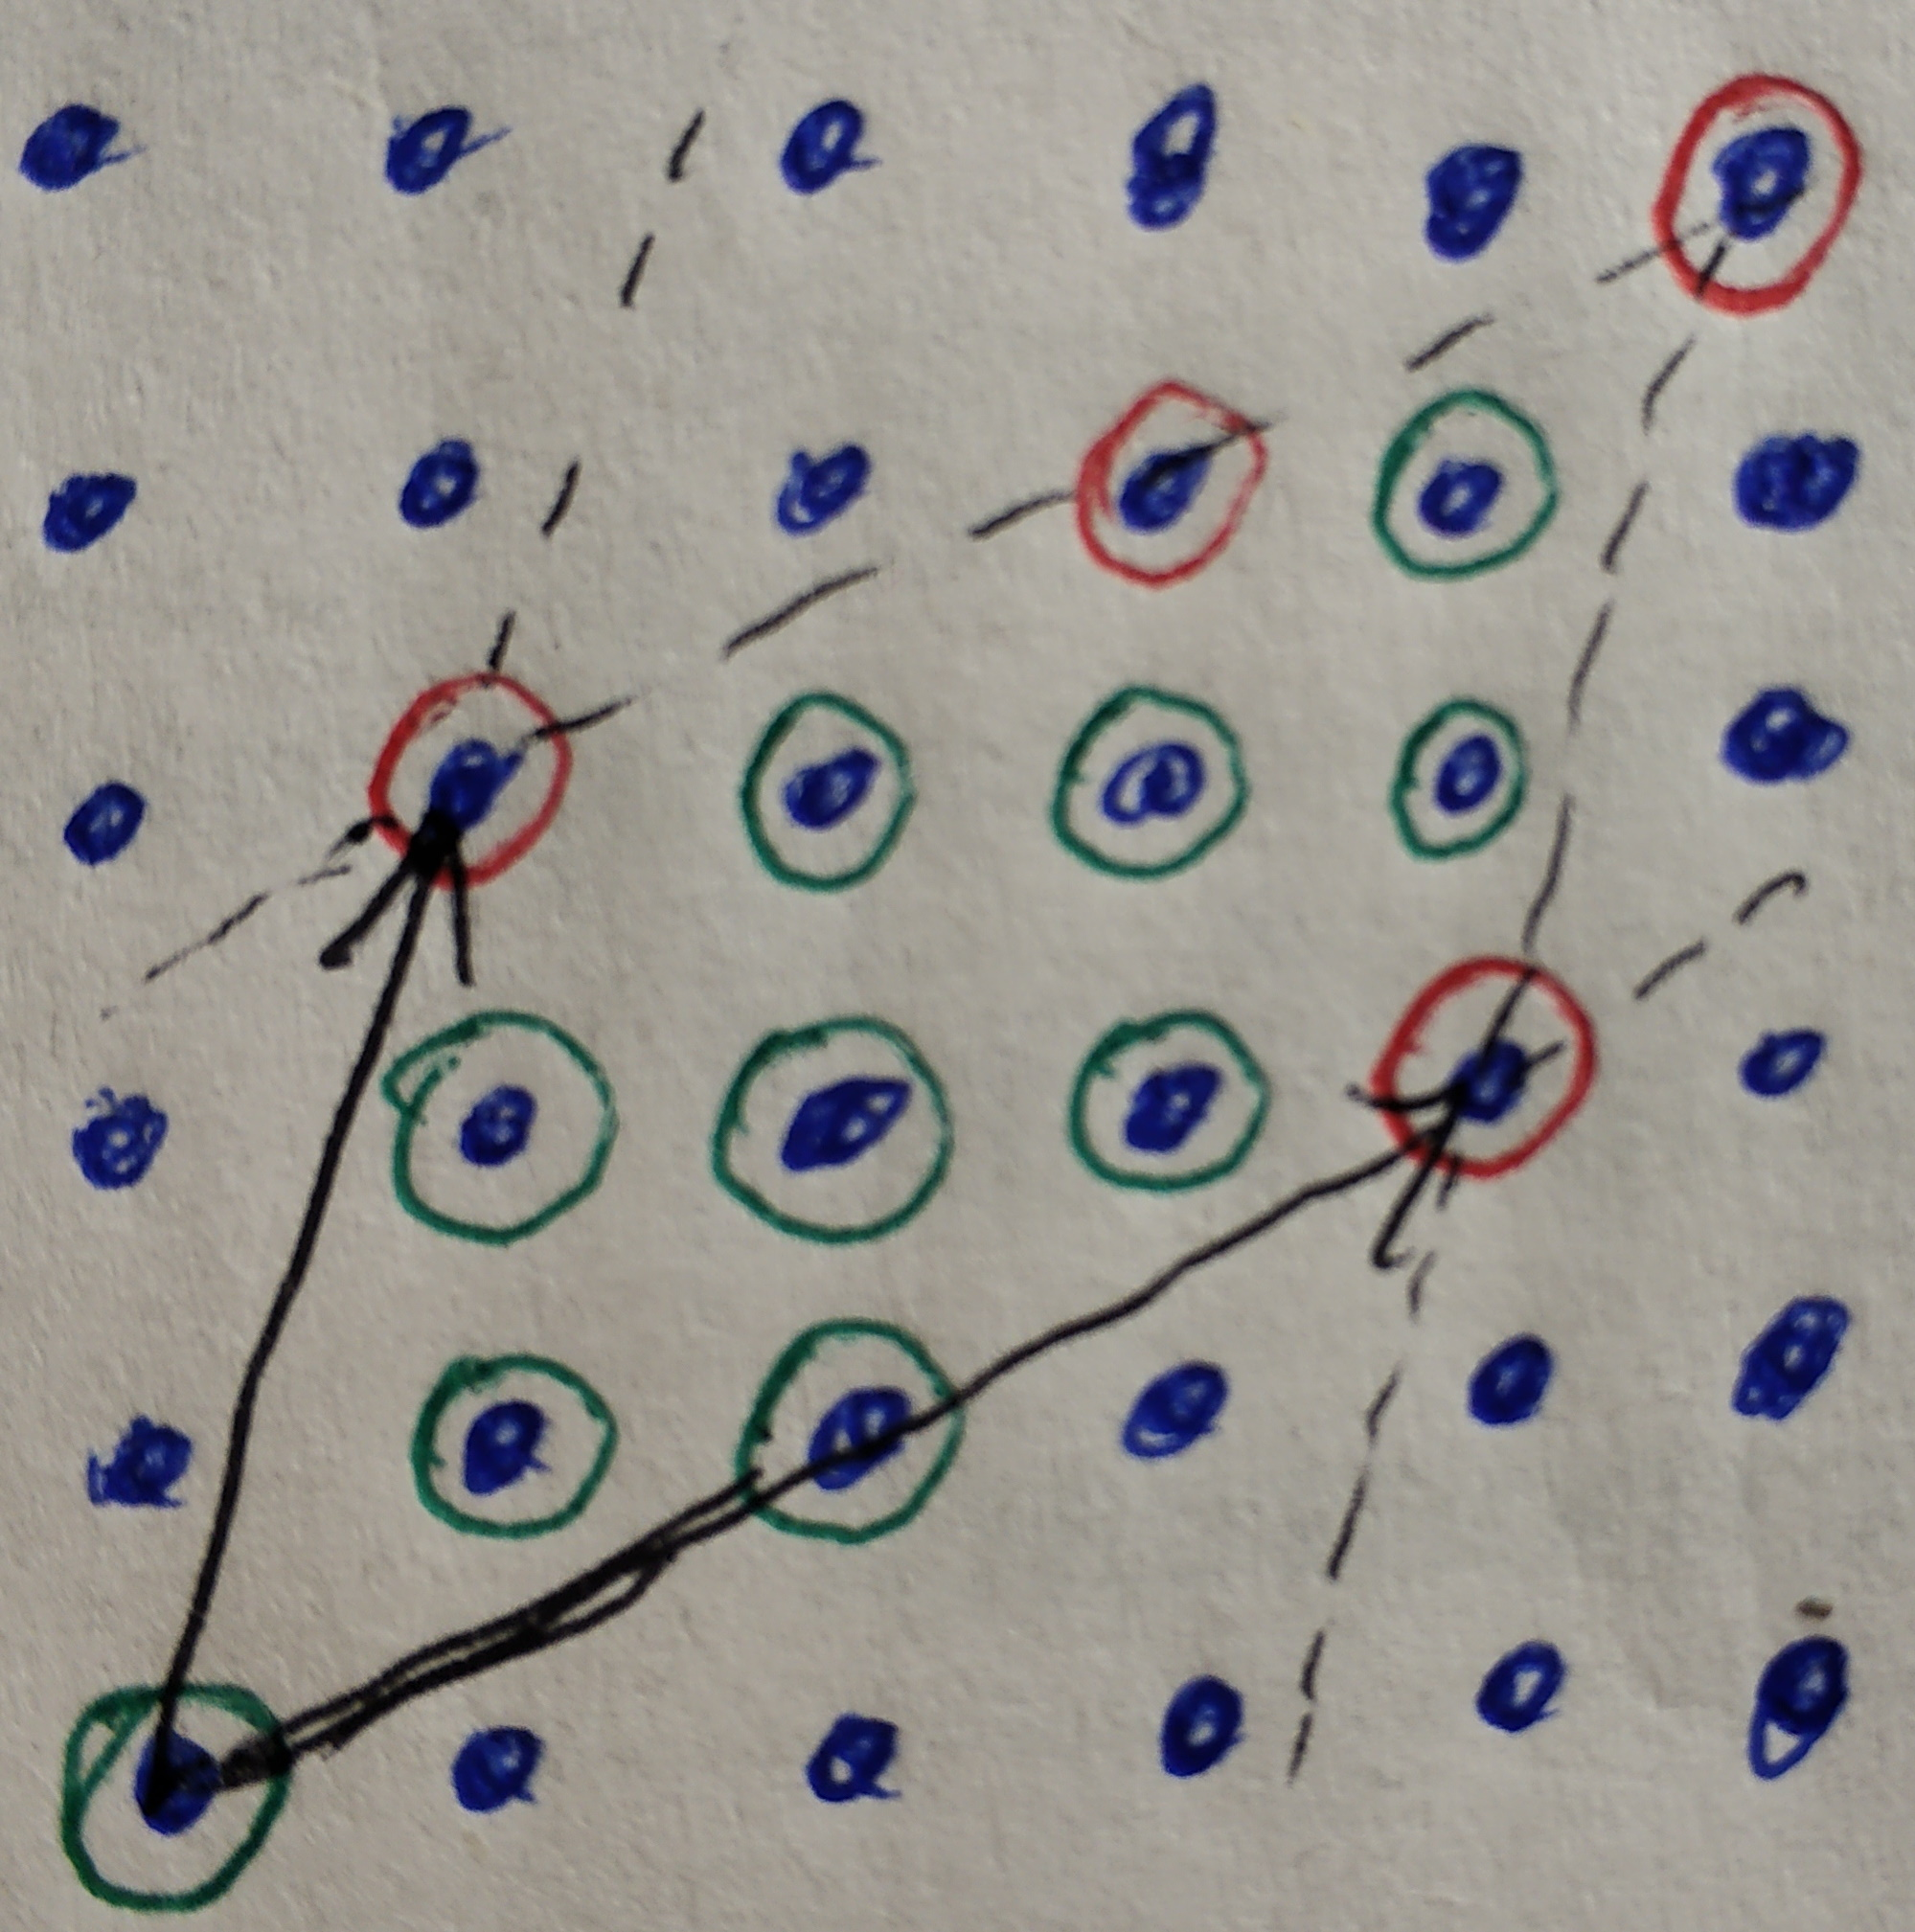
\includegraphics[height=5cm]{TI-HW-006-3.jpg}
                        \caption{Чёрное --- два вектора и решётка, порождённая ими. Зелёное --- остатки по модулю решётки, красное --- НЕ остатки по модулю решётки.}
                    \end{figure}
                    Пусть $t$ --- какой-то остаток по модулю решётки. Заметим, что если вектор $h \equiv t \pmod{q_1, q_2}$ лежит в $\sum_{i=1}^k \{u_i\}^*$, то
                    \[h = v + \sum_{i=1}^k a_i u_i\]
                    для некоторых $a_i \in \NN \cup \{0\}$. Тогда $h + b_1 q_1 + b_2 q_2$ для всех $b_1, b_2 \in \NN \cup \{0\}$ тоже получается выражением. Рассмотрим в квадранте, натянутом на $q_1$ и $q_2$, все квадратики (клетки), где реализуется этот остаток $t$ в $\sum_{i=1}^k \{u_i\}^*$.
                    \begin{figure}[H]
                        \centering
                        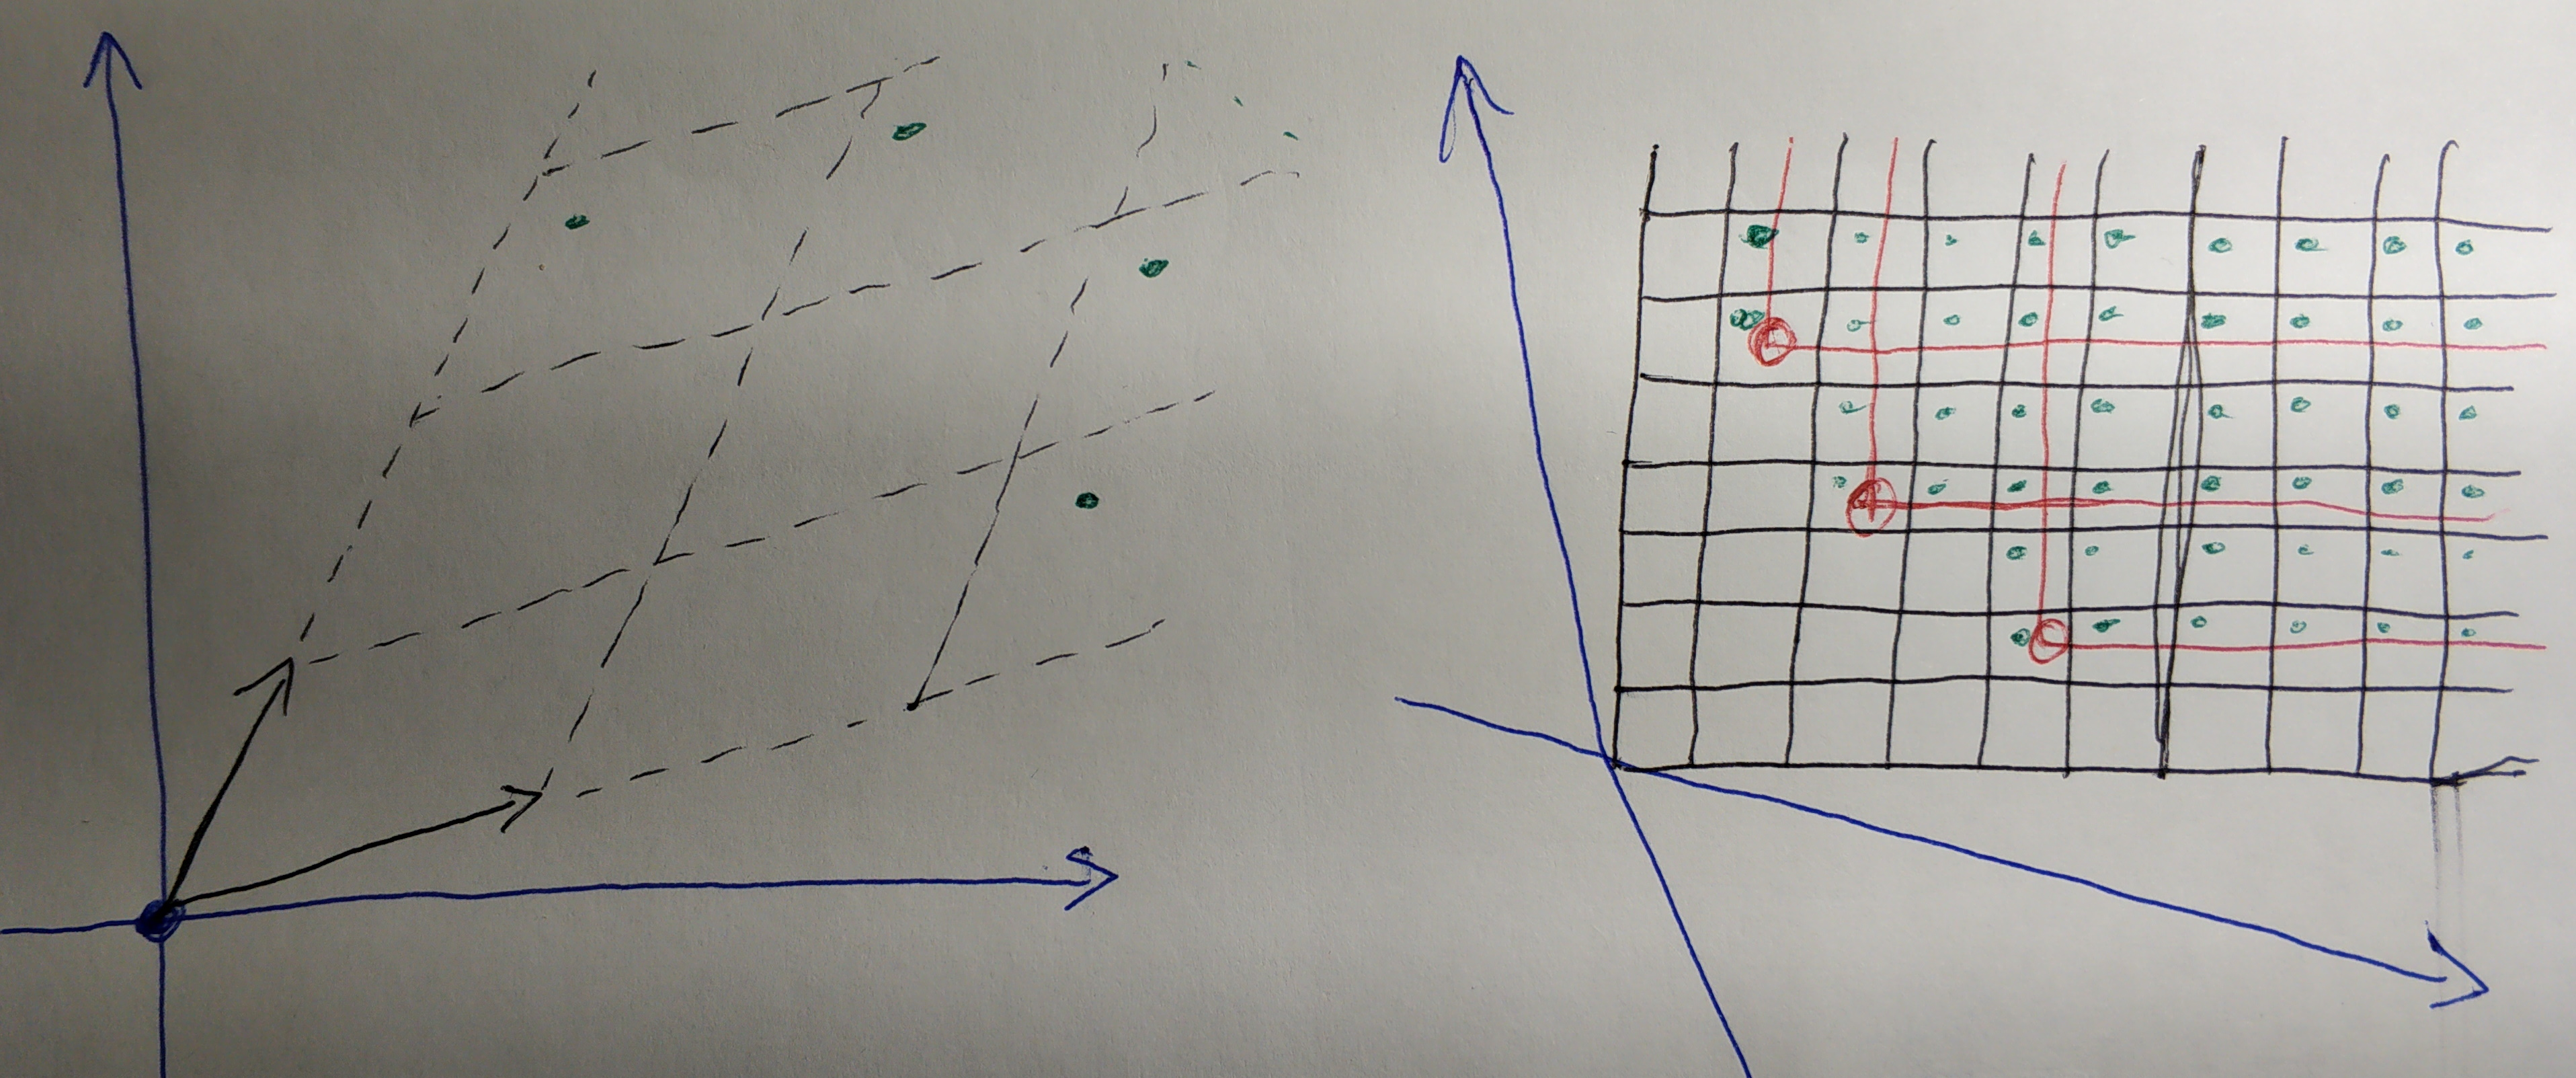
\includegraphics[height=5cm]{TI-HW-006-4.jpg}
                        \caption{Зелёным слева и справа отмечены появления фиксированного остатка в множестве, заданным выражением. Слева --- со стороны обычной плоскости $\ZZ^2$, справа --- со стороны квадранта, натянутого на $q_1$ и $q_2$.}
                    \end{figure}
                    Из выше сказанного следует, что если в какой-то клеточке реализуется остаток, то он реализеутся и во всех клетках выше и правее. Поэтому можно выделить конечный набор клеток в квадранте, что множество всех клеток с реализацией остатка есть объединение квадрантов с центрами в клетках из этого конечного набора (для примера см. рисунок выше).

                    Обозначим для всякого остатка $t$
                    \[S_t := \left\{h \in \sum_{i=1}^k \{u_i\}^* \mid h \equiv t \pmod{q_1, q_2}\right\}.\]
                    Тогда мы показали, что $S_t$ раскладывается в конечное объединение множеств, задающихся выражениями вида $\{p\} + \{q_1\}^* + \{q_2\}^*$, где $p$ --- те самые элементы только что выделенного конечного множества. Поскольку остатков конечное количество, то множеств $S_t$ конечно, а значит всё множество раскладывается так, как мы захотели.

                    Если же $q_1$ и $q_2$ коллинеарны, то все $u_i$ коллинеарны. Тогда переобозначим $q_1$ в $q$, а про $q_2$ забудем. Тогда рассмотрим вектора на луче $q \cdot \RR_{\geqslant 0}$, лежащие во множестве $\sum_{i=1}^k \{u_i\}^*$. Опять рассмотрим остатки на этом луче по модулю $q$. Получится аналогичная картинка, но не с двумерным квадрантом, а с одномерным: точно также для всякого остатка $t$ будет первая клетка, лежащая в $\sum_{i=1}^k \{u_i\}^*$, а вместе с ней будут лежать и все последующие клетки. Тогда
                    \[S_t := \left\{h \in \sum_{i=1}^k \{u_i\}^* \mid h \equiv t \pmod{q}\right\}\]
                    представляется в виде $\{v_t\} + \{q\}^*$ для некоторого $v_t$. А тогда
                    \[\sum_{i=1}^k \{u_i\}^* = \sum_{t} S_t = \sum_t \{v_t\} + \{q\}^* + \{(0; 0)\}^*.\]
                \end{proof}

                \begin{corollary}\label{RE-2-normal-form}
                    Всякое выражение как в \ref{RE-normal-form} упрощается без изменения значения до выражения вида
                    \[
                        (E_1) \cup \dots \cup (E_n),
                        \qquad \text{ где } \qquad
                        E_i = \{v_i\} + \{u_{i, 1}\}^* + \{u_{i, 2}\}^*,
                    \]
                    где $v_i$ и $u_{i, j}$ --- некоторые вектора из $(\NN \cup \{0\})^2$, $n \geqslant 1$.
                \end{corollary}

                \begin{proof}
                    Поскольку по лемме каждый из термов $E_i$ выражения как в \ref{RE-normal-form} можно представить в виде выражения как в \ref{RE-2-normal-form}, то объединение этих выражений (без дополнительных скобок) будет выражение как в \ref{RE-2-normal-form}.
                \end{proof}

                \begin{corollary}
                    TFAE
                    \begin{itemize}
                        \item Для всякого выражения $t$ как в \ref{RE-normal-form} язык $L(t)$ грамматизируется.
                        \item Для всякого выражения $t$ как в \ref{RE-2-normal-form} язык $L(t)$ грамматизируется.
                    \end{itemize}
                \end{corollary}

                \begin{proof}
                    Если верно первое утверждение, то всякое выражение $t$ как в \ref{RE-2-normal-form} является выражением как в \ref{RE-normal-form}, а тогда $L(t)$ грамматизируется.

                    Если верно второе, то для всякого выражения $t$ как в \ref{RE-normal-form} есть выражение $t'$ как в \ref{RE-2-normal-form} с тем же значением. Тогда $L(t) = L(S(t)) = L(S(t')) = L(t')$ грамматизируется.
                \end{proof}

                \begin{lemma}
                    TFAE
                    \begin{itemize}
                        \item Для всякого выражения $t$ как в \ref{RE-2-normal-form} язык $L(t)$ грамматизируется.
                        \item Для всякого выражения $t$ вида $\{p\} + \{q_1\}^* + \{q_2\}^*$ язык $L(t)$ грамматизируется.
                    \end{itemize}
                \end{lemma}

                \begin{proof}
                    Если верно первое утверждение, то всякое выражение $t$ вида $\{p\} + \{q_1\}^* + \{q_2\}^*$ является выражением как в \ref{RE-2-normal-form}, а значит $L(t)$ грамматизируется.

                    Если верно второе утверждение, то для всякого выражения $t$ как в \ref{RE-2-normal-form} есть набор выражений $t'_1$, \dots, $t'_n$ вида $\{p\} + \{q_1\}^* + \{q_2\}^*$, что $t = (t'_1) \cup \dots \cup (t'_n)$. Следовательно, каждый язык $L(t'_i)$ грамматизируется. А тогда и
                    \[
                        L(t)
                        = L(S(t))
                        = L(S(t'_1) \cup \dots \cup S(t'_n))
                        = L(S(t'_1)) \cup \dots \cup L(S(t'_n))
                        = L(t'_1) \cup \dots \cup L(t'_n)
                    \]
                    грамматизируется (конечное объединение грамматизируемых языков грамматизируемо).
                \end{proof}

                Теперь сделаем ещё одно упрощение.

                \begin{definition}
                    \emph{Cлияние} двух строк $v$ и $u$ --- такая строка $w$, что есть некоторые разбиения $v = v_1\dots v_n$ и $u = u_1\dots u_n$ (каждая из $v_i$ и $u_i$ может оказаться пустой), что $w = v_1 u_1 \dots v_n u_n$. Обозначим множество всех слияний строк $v$ и $u$ за $v \diamond u$.

                    Также обобщим операцию на языки:
                    \[
                        v \diamond L := \bigcup_{u \in L} v \diamond u,
                        \qquad
                        L \diamond v := \bigcup_{u \in L} u \diamond v,
                        \qquad
                        M \diamond L := \bigcup_{\substack{v \in M\\u \in L}} v \diamond u.
                    \]
                \end{definition}

                \begin{lemma}\ 
                    \begin{enumerate}
                        \item Операция $\diamond$ коммутативна.
                        \item Для любого разбиения $v = v_1 \dots v_n$ и любого слова $u$ верно
                            \[(v_1 \dots v_n) \diamond u = \bigcup_{u_1 \dots u_n = u} (v_1 \diamond u_1) \dots (v_n \diamond u_n),\]
                            где итерация в объединении ведётся по всем разбиениям $u$.
                        \item Для всяких множеств векторов $V$ и $U$ верно $L(V + U) = L(V) \diamond L(U)$.
                        \item Пусть даны язык $L$, задающийся грамматикой, и некоторое слово $v$. Тогда язык $v \diamond L$ задаётся грамматикой.
                        \item Пусть даны язык $L$, задаваемый грамматикой, и конечный язык $M$. Тогда $M \diamond L$ задаётся грамматикой.
                    \end{enumerate}
                \end{lemma}

                \begin{proof}
                    \begin{enumerate}
                        \item Пусть $w \in v \diamond u$. Тогда $w = v_1 u_1 \dots v_n u_n$, где $v = v_1 \dots v_n$, $u = u_1 \dots u_n$. Тогда $w = \varepsilon v_1 \dots u_{n-1} v_n u_n \varepsilon$, где $u = \varepsilon u_1 \dots u_n$, $v = v_1 \dots v_n \varepsilon$, т.е. $w \in u \diamond v$. Т.е. $v \diamond u \subseteq u \diamond v$. Аналогично $u \diamond v \subseteq v \diamond u$.
                        \item Несложно видеть из определения, что $(v_1 \diamond u_1) (v_2 \diamond u_2) \subseteq (v_1 v_2) \diamond (u_1 u_2)$. Следовательно,
                            \[\bigcup_{u_1 \dots u_n = u} (v_1 \diamond u_1) \dots (v_n \diamond u_n) \subseteq (v_1 \dots v_n) \diamond u,\]
                            так как для каждого разбиения $u = u_1 \dots u_n$ верно
                            \[(v_1 \diamond u_1) \dots (v_n \diamond u_n) \subseteq (v_1 \dots v_n) \diamond (u_1 \dots u_n) = (v_1 \dots v_n) \diamond u.\]
                            Теперь покажем обратное утверждение.

                            Пусть $w \in (v_1 \dots v_n) \diamond u$. Расскрасим символы $w$ в два цвета: символы от слова $v_1 \dots v_n$ покрасим в белый, а все остальные в чёрный. Тогда подстрока $w$, состоящая из белых символов, образует слово $v_1 \dots v_n$, а из всех чёрных --- $u$. Пометим в белой подстроке буквы, являющиеся первыми буквами подслов $v_i$ и разделим строку $w$ по промежуткам перед отмеченными буквами. Получим разбиение $w = w_1 \dots w_n$. Заметим, что чёрные подстроки в каждом $w_i$ являются словами $v_i$. Пусть $u_i$ --- белая подстрока в $w_i$. Тогда $w_i \in v_i \diamond u_i$. При этом $u_1 \dots u_n$ образует белую подстроку $w_1 \dots w_n = w$, т.е. $u$. Следовательно
                            \[w \in (v_1 \diamond u_1) \dots (v_n \diamond u_n),\]
                            где $u_1 \dots u_n$ --- некоторое разбиение $u$. Следовательно,
                            \[(v_1 \dots v_n) \diamond u \subseteq \bigcup_{u_1 \dots u_n = u} (v_1 \diamond u_1) \dots (v_n \diamond u_n).\]
                        \item Пусть $w \in L(V) \diamond L(U)$. Тогда есть $v \in L(V)$ и $u \in L(U)$, что $w \in v \diamond u$. Тогда $\overline{w} = \overline{v} + \overline{u}$. При этом $\overline{v} \in V$, а $\overline{u} \in U$, т.е. $\overline{w} \in V + U$. Следовательно $w \in L(V + U)$.
                        
                            Если $w \in L(v + u)$, то $\overline{w} \in V + U$, а тогда есть $p \in V$ и $q \in U$, что $\overline{w} = p + q$. Тогда выделим в $w$ любой набор символов, описывающий вектор $p$. Тогда выделенные слова образуют подстроку $v$, а оставшиеся --- $u$. Это значит, что $\overline{v} = p$, а $\overline{u} = q$, и $w \in v \diamond u$. Т.е. $v \in L(V)$, $u \in L(U)$, а тогда $w \in L(V) \diamond L(U)$.
                        \item Пусть дана грамматика $(\Sigma, N, R, S)$, порождающая $L$. Рассмотрим новую грамматику $(\Sigma, N', R', S')$, где
                            \begin{itemize}
                                \item $N'$ --- множество символов $A_u$ (копий $A$) для каждого $A \in N$ и подслова $u$ слова $v$.
                                \item $R'$ состоит из правил полученных следующим образом. Пусть имеется правило
                                    \[A \to w_0 B_1 \dots B_n w_n,\]
                                    где $w_i \in \Sigma^*$, $B_i \in N$. Тогда добавим в $R'$ все возможные правила
                                    \[A_u \to w'_0 (B_1)_{y_1} \dots (B_n)_{y_n} w'_n,\]
                                    где $w'_i \in w_i \diamond x_i$, для всех разбиений $u = x_0 y_1 x_1 \dots y_n x_n$.
                                \item $S' := S_v$.
                            \end{itemize}
                            Покажем, что данная грамматика порождает $v \diamond L$.
        
                            Докажем, что если $w$ порождено $A_u$, то $w \in u \diamond L(A)$, по (полной) индукции одновременно по размеру дерева разбора $w$ и по $|u|$.
                            
                            Рассмотрим первую подстановку в дереве разбора $w$. Это правило
                            \[A_u \to w'_0 (B_1)_{y_1} \dots (B_n)_{y_n} w'_n\]
                            для некоторых $w'_i \in w_i \diamond x_i$ и некоторого разбиения $u = x_0 y_1 x_1 \dots y_n x_n$. По предположению индукции $(B_i)_{y_i}$ (им можно воспользоваться, так как поддерево $(B_i)_{y_i}$ имеет строго меньший размер, а $|y_i| \leqslant |u|$) будет заменено на какое-то слово $b_i \in y_i \diamond L(B_i)$. Т.е.
                            \begin{align*}
                                w
                                &= w'_0 b_1 \dots b_n w'_n\\
                                &\in (x_0 \diamond w_0) (y_1 \diamond L(B_1)) \dots (y_n \diamond L(B_n)) (x_n \diamond w_n)\\
                                &\subseteq (x_0 y_1 x_1 \dots y_n x_n) \diamond (w_0 L(B_1) \dots L(B_n) w_n)\\
                                &= u \diamond (w_0 L(B_1) \dots L(B_n) w_n).
                            \end{align*}
                            Но так как (в изначальной грамматике) имеется правило
                            \[A \to w_0 B_1 \dots B_n w_n,\]
                            значит
                            \[w_0 L(B_1) \dots L(B_n) w_n \subseteq L(A),\]
                            т.е. $w \in u \diamond L(A)$.
        
                            Теперь покажем, что всякое слово из $w \diamond u$, где $w \in L(A)$, порождается символом $A_u$ по индукции одновременно по размеру дерева разбора $w$ и $|u|$.
                            
                            Пусть первое правило в дереве разбора $w$ --- это
                            \[A \to w_0 B_1 \dots B_n w_n.\]
                            Тогда слово $w$ разбивается как $w_0 b_1 \dots b_n w_n$, где $b_i$ порождается $B_i$. Тогда для вяского слова $z \in w \diamond u$ есть разбиение $u = x_0 y_1 \dots y_n x_n$, что
                            \[z \in (x_0 \diamond w_0) (y_1 \diamond b_1) \dots (y_n \diamond b_n) (x_n \diamond w_n).\]
                            По предположению индукции $y_i \diamond b_i$ порождается $(B_i)_{y_i}$ (так как у $b_i$ дерево разбора строго меньше, а $|y_i| \leqslant |u|$). Значит $z$ можно получить из $A_u$, где первой подстановкой будет
                            \[A_u \to w'_0 (B_1)_{y_1} \dots (B_n)_{y_n} w'_n,\]
                            где $w'_i$ --- слово из $x_i \diamond w_i$, соответствующее $z$, а дальше на каждом $(B_i)_{y_i}$ повиснет дерево разбора для соответствующего куска $z$. Т.е. $z \in L(A_u)$.
        
                            Поскольку мы начинаем в $S_v$, то язык, порождаемый новой грамматикой есть $v \diamond L(S) = v \diamond L$.
                        \item Поскольку
                            \[M \diamond L = \bigcup_{v \in M} v \diamond L,\]
                            каждый язык $v \diamond L$ грамматизируется, а объединение конечно, то и весь $M \diamond L$ грамматизируется.
                    \end{enumerate}
                \end{proof}

                \begin{corollary}
                    TFAE
                    \begin{itemize}
                        \item Для всякого выражения $t$ вида $\{p\} + \{q_1\}^* + \{q_2\}^*$ язык $L(t)$ грамматизируется.
                        \item Для всякого выражения $t$ вида $\{q_1\}^* + \{q_2\}^*$ язык $L(t)$ грамматизируется.
                    \end{itemize}
                \end{corollary}

                \begin{proof}
                    Если верно первое, то всякое выражения $t$ вида $\{q_1\}^* + \{q_2\}^*$ имеет вид $\{p\} + \{q_1\}^* + \{q_2\}^*$ (просто вставить $p = (0; 0)$), а значит $L(t)$ грамматизируется.

                    Если верно второе, то всякое выражение $t$ вида $\{p\} + \{q_1\}^* + \{q_2\}^*$ можно представить $s + r$, где $s := \{p\}$, $r := \{q_1\}^* + \{q_2\}^*$. Тогда $L(r)$ грамматизируется, а $L(s)$ конечно. А значит и
                    \[L(t) = L(S(s + r)) = L(S(s) + S(r)) = L(S(s)) \diamond L(S(r)) = L(s) \diamond L(r)\]
                    грамматизируем.
                \end{proof}

                \begin{remark*}
                    Выражения $\{q_1\}^* + \{q_2\}^*$ и $\{q_1; q_2\}^*$ значат одно и то же. Поэтому мы будем на лету использовать то одно выражение, то другое.
                \end{remark*}

                Мы долго изменяли задачу, упрощая условие, но оставаясь в равносильной области. Теперь перейдём в атаку: будем показывать, что все такие языки задаются грамматиками.

                \begin{definition}
                    Назовём \emph{зацикленным словом} слово с точностью до циклических сдвигов (но не разворотов!). Т.е. фактически это класс слов, получающихся друг из друга циклическими сдвигами. Множества зацикленных слов будем называть \emph{зацикленными языками}.

                    Назовём \emph{зациклением} слова $w$ соответствующее ему зацикленное слово, которое будем обозначать $w^\circ$. Тогда для всякого языка $M$ будем называть \emph{зациклением} языка $M$ зацикленный язык
                    \[L^\circ(M) := \{w^\circ\}_{w \in M}\]
                    (если это не приведёт к путанице, можно также писать $M^\circ$).

                    Назовём \emph{разрыванием} зацикленного слова $\omega$ всякое слово $w$, что $\omega$ является зацикливанием $w$:
                    \[\omega = w^\circ\]
                    (и, фактически, $w \in \omega$). Тогда назовём \emph{языком (всевозможных) разрываний} зацикленного слова $\omega$ язык состоящий из всех разрываний $\omega$:
                    \[L(\omega) := \{w \in \Sigma^* \mid w^\circ = \omega\}\]
                    (опять же, фактически, $L(\omega) = \omega$). Также назовём \emph{языком (всевозможных) разрываний} зацикленного языка $M$ язык
                    \[L(M) := \bigcup_{\omega \in M} L(\omega).\]
                \end{definition}

                \begin{definition}
                    Пусть дан язык $M$. Определим \emph{язык вставок} языка $M$ как язык $\Insertion(M)$, состоящий из слов, полученных из $\varepsilon$, в которую конечное число раз вставили в абсолютно любое место (в том числе с краю) некоторую строку из $M$.
                    
                    Пусть дан язык $M$. Определим \emph{зацикленный язык вставок} языка $M$ как зацикленный язык $\Insertioncirc(M)$, состоящий из слов, полученных из зацикленной $\varepsilon$, в которую конечное число раз вставили в абсолютно любое место некоторую строку из $M$.
                \end{definition}

                \begin{lemma}
                    Для всяких векторов $q_1$ и $q_2$ есть конечный набор векторов $S \subseteq \{q_1; q_2\}^* \setminus \{(0; 0)\}$, что во всяком непустом зацикленном слове из $L^\circ(\{q_1; q_2\}^*)$ есть подслово с вектором из $S$.
                \end{lemma}

                \begin{proof}
                    Фиксируем какое-нибудь зацикленное слово $w$ и какой-нибудь вектор $(k; l)$. Будем рассматривать всевозможные подслова слова $w$ длины ровно $k + l$. Если перейти от какого-либо подслова к следующему (сдвинуть область (не сами символы) из $k+l$ последовательных символов влево или вправо по слову $w$), то количество символов $a$ либо не изменится, либо изменится на $\pm 1$. Значит если в $w$ нет подслова с вектором $(k; l)$, то в каждом подслове длины $k+l$ либо строго меньше $k$ символов $a$, либо строго больше $k$, так как если есть оба, то дискретной непрерывности будет подслово с ровно $k$ буквами $a$.

                    Пусть в слове $A$ букв $a$ и $B$ букв $b$. Тогда просуммируем количества букв $a$ в каждом подслове из $k+l$ элементов. Тогда каждая буква $a$ была посчитана $k+l$ раз, а значит сумма равна $A(k+l)$. С другой стороны либо во всех подсловах $\leqslant k-1$ буквы $a$, либо $\geqslant k+1$, т.е.
                    \begin{gather*}
                        \text{либо } A(k+l) \leqslant (A+B)(k-1),
                        \qquad
                        \text{либо } A(k+l) \geqslant (A+B)(k+1),\\
                        \text{т.е. либо } \frac{A}{A+B} \leqslant \frac{k-1}{k+l},
                        \qquad
                        \text{либо } \frac{A}{A+B} \geqslant \frac{k+1}{k+l}.
                    \end{gather*}
                    Также заметим, что это утверждение верно только если $A+B \geqslant k+l$.

                    Это утверждение значит, что если $A+B \geqslant k+l$ и $\frac{k-1}{k+l} < \frac{A}{A+B} < \frac{k+1}{k+l}$, то в зацикленном слове с вектором $(A; B)$ найдётся подслово с вектором $(k; l)$. Т.е. если изображать это на рисунке, то получится как на рис. ниже (слева). Мы отложили вектора $(k+1; l-1)$ и $(k-1; l+1)$. Все вектора, находящиеся в верхней полуплоскости относительной прямой через эти два вектора, --- это ровно все вектора $(A; B)$, что $A+B \geqslant k+l$, и только. При этом вектора находящиеся между прямыми, являющимися продолжениями $(k+1; l-1)$ и $(k-1; l+1)$ --- это ровно все вектора $(A; B)$, что $\frac{k-1}{k+l} < \frac{A}{A+B} < \frac{k+1}{k+l}$. Следовательно нам нужна крассная область.
                    \begin{figure}[H]
                        \centering
                        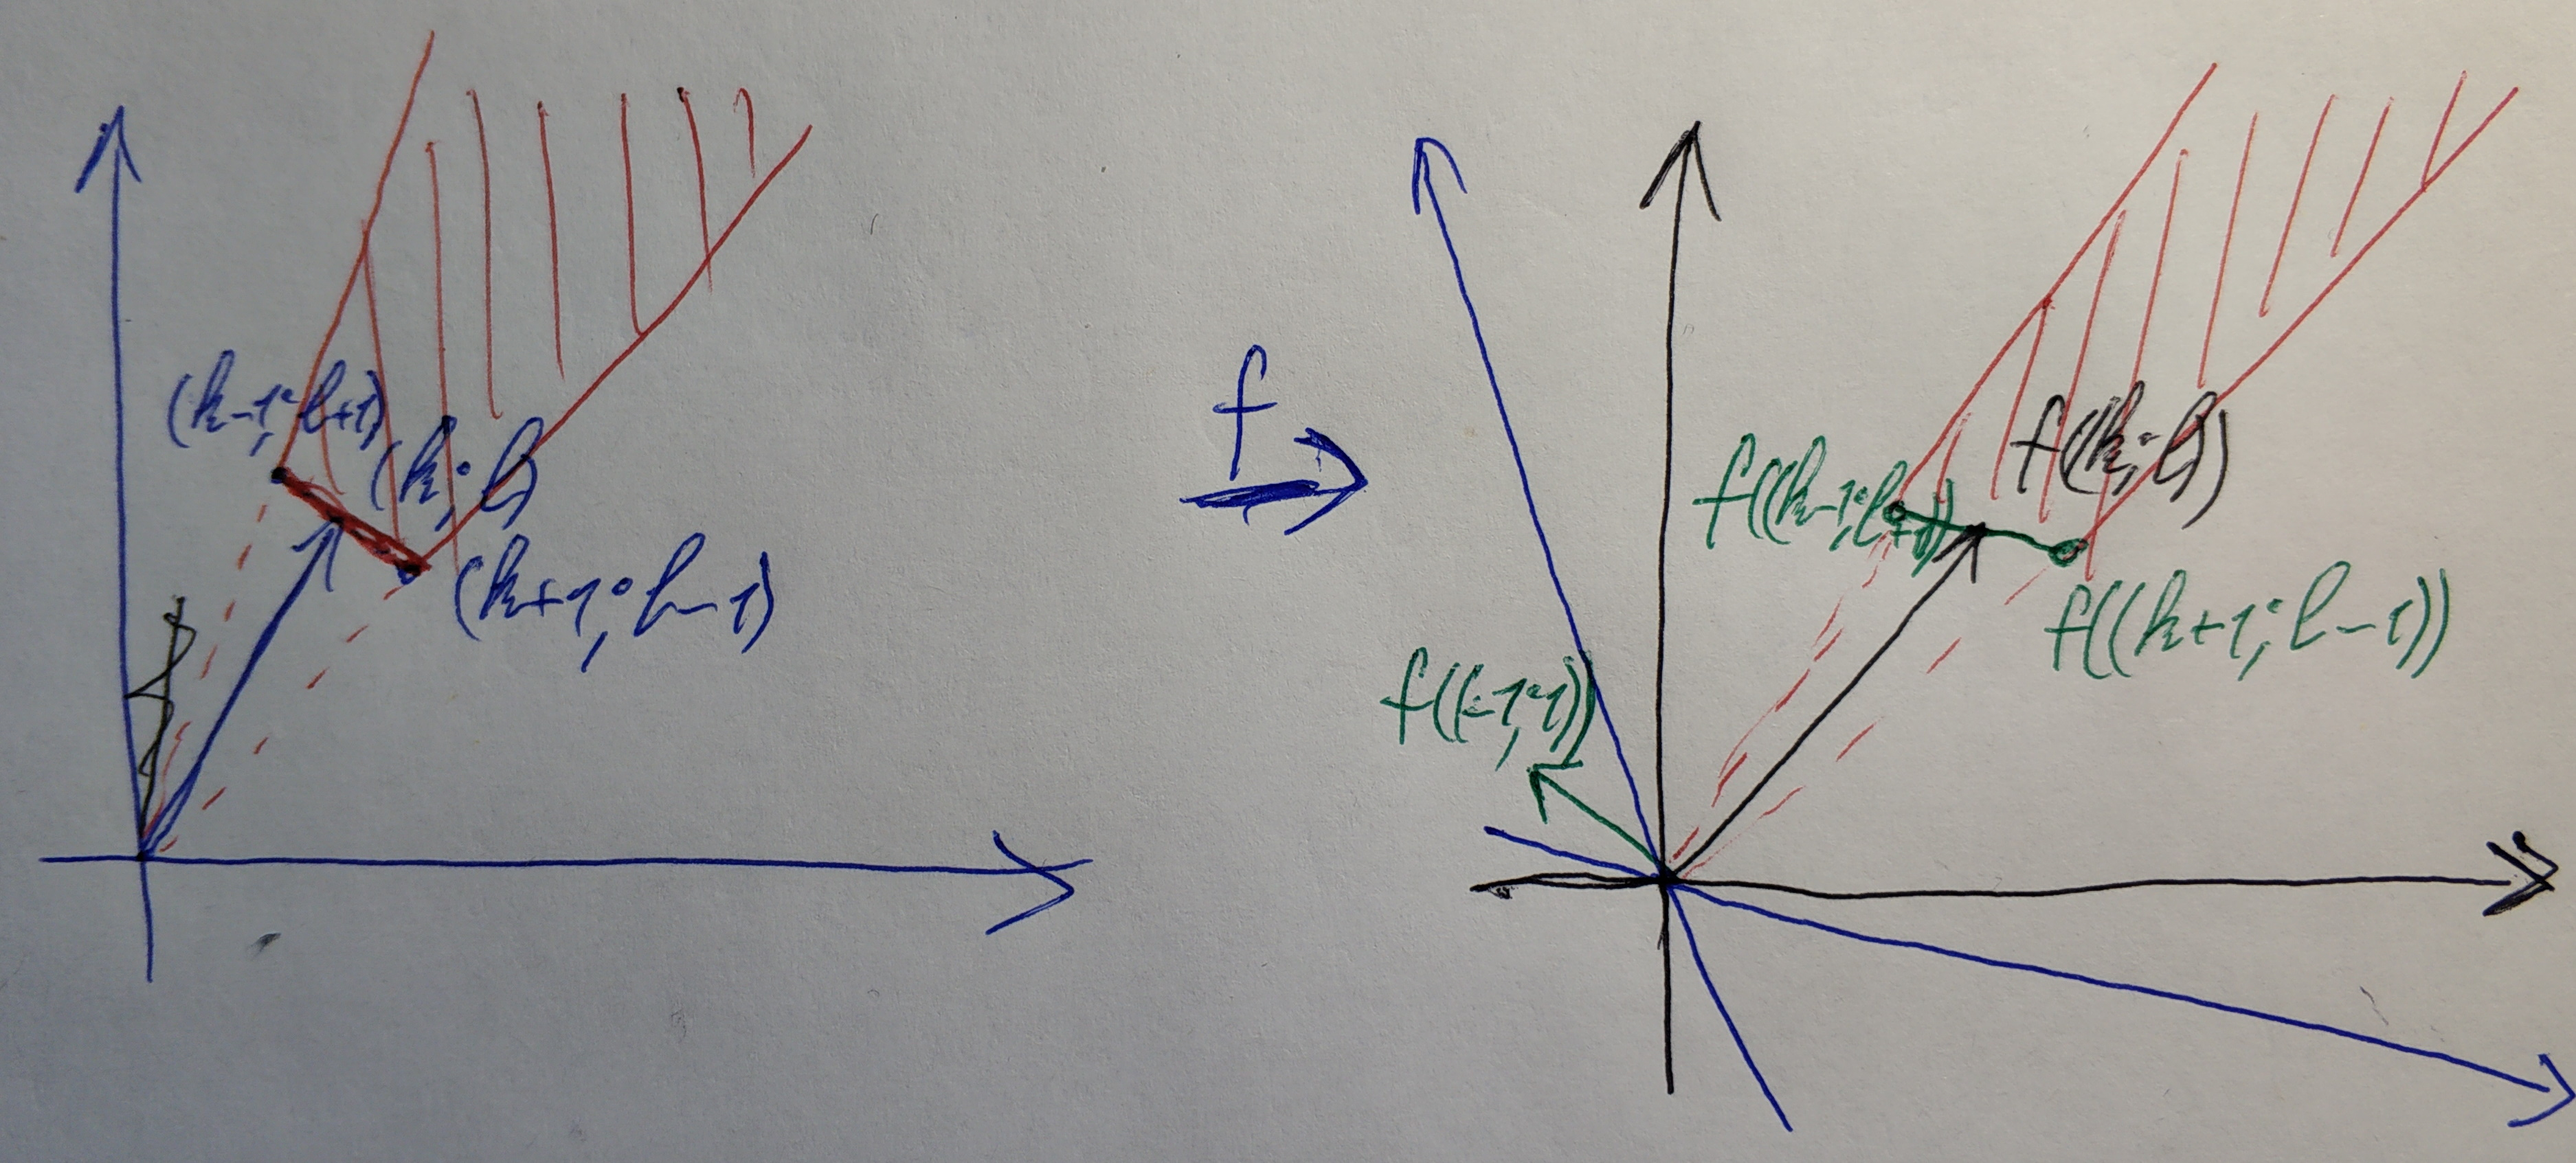
\includegraphics[height=5cm]{TI-HW-006-5.jpg}
                        \caption{Слева --- картинка в обычном базисе, справа --- в базисе $\{q_1; q_2\}$. Крассная область --- область хороших для $(k; l)$ (и его образа) векторов, т.е. тех для которых точно верно условие, что есть подслово вектора $(k; l)$. Причём интервал между векторами $(k; l) \pm 1$ включается, а две другие бесконечные стороны красной области из неё исключаются.}
                    \end{figure}
                    
                    Теперь давайте перейдём в базис $(q_1; q_2)$ и будем рассматривать только слова $w \in L(\{q_1; q_2\}^*)$. Понятно, что у всех таких слов $w$ вектора в новом базисе имеют координаты из $(\NN \cup \{0\})^2$ (причём все возможные). Теперь красная область (область векторов, удовлетворяющих условию для $(k; l)$) строится также, но от $(k; l)$ теперь надо откладывать не $\pm (1; -1)$, а его образ $\delta$; несложно видеть, что он имеет вид $\delta = (c;d)$, где $c > 0$, а $d < 0$, так как четвёртый квадрант в старом базисе лежит внутри четвёртого квадранта в новом базисе.

                    Временно не будем ограничивать красную область прямой через вектора $(k; l) \pm \delta$, т.е. будем брать полный угол между векторами (точнее его внутренность). Давайте рассмотрим прямую $x+y = 1$ и будем проецировать всё на неё через центр координат. Также введём на ней локальные аффинные координаты так, что $(1;0)$ будем иметь координату $1$, а $(0; 1)$ --- $0$. Тогда всякий вектор $(k; l)$ спроецируется в координату $\frac{k}{k+l}$. Также всякая рациональная координата $\frac{n}{m} \in [0; 1]$ реаализуется вектором $(n; m - n) \in (\NN \cup \{0\})^2$.
                    
                    Хотим понять, а какую окрестность $(k; l)$ спроецируется угол между векторами $(k; l) \pm \delta$. Уменьшим длину вектора $(c; d)$ так, чтобы $|c| + |d| = c-d < \frac{1}{2}$, а значит $|c + d| < \frac{1}{2}$. Тогда область-угол у каждого вектора не увеличиться, но и не будет содержать вектора с прямой $x=y$ даже на границе, т.е. проекция этого угла будет ограниченным интервалом. $(k + c; l + d)$ спроецируется в $\frac{k+c}{k+l+c+d}$. Значит
                    \[
                        \frac{k+c}{k+l+c+d} - \frac{k}{k+l}
                        = \frac{(k+c)(k+l) - k(k+l+c+d)}{(k+l+c+d)(k+l)}
                        = \frac{1}{k+l} \cdot \frac{lc - kd}{k+l+c+d}.
                    \]
                    При этом $c \geqslant 1$ и $-d \geqslant 1$, поэтому $lc - kd \geqslant k+l$, а $|c+d| \leqslant \frac{1}{2} \leqslant \frac{1}{2}(k+l)$, значит $k+l+c+d \geqslant (k+l) - |c+d| \geqslant \frac{1}{2}(k+l)$, а значит
                    \[\frac{k+c}{k+l+c+d} - \frac{k}{k+l} \geqslant \frac{1}{2(k+l)}.\]
                    Аналогично получается, что
                    \[\frac{k-c}{k+l-c-d} - \frac{k}{k+l} \leqslant -\frac{1}{2(k+l)}.\]
                    Т.е. у всякой рациональной точки $n/m \in [0; 1]$ красный угол $(n; m-n)$ проецируется в множество, содержащее $1/2m$-окрестность точки $(n/m)$. Рассмотрим семейство этих окрестностей.

                    По теореме Гурвица у всякого $\alpha \in (0; 1)$ есть бесконечно много рациональных чисел $n/m$, что
                    \[
                        \left|\alpha - \frac{n}{m}\right| < \frac{1}{m^2}.
                    \]
                    Тогда можно поставить условие $\frac{n}{m} \in [0; 1]$ и $m \geqslant 2$ и теорема останется верна. Но тогда
                    \[
                        \left|\alpha - \frac{n}{m}\right| < \frac{1}{m^2} \leqslant \frac{1}{2m}.
                    \]
                    Т.е. всякое $\alpha \in [0; 1]$ покрывается хоть одной такой окрестностью. Тогда по компактности отрезка $[0; 1]$ его покрывает и какой-то конечный поднабор окрестностей. Т.е. есть конечный набор векторов $(k; l)$, что соответствующие им красные углы покрывают весь первый квадрант.

                    Если вспомнить, что у углов нужно отрезать ещё небольшой треугольничек, то непокрытыми останутся конечное количество точек, тогда их можно просто добавить к набору выбранных векторов. Таким обарзом мы сконструировали конечный набор векторов, что у всякого непустого слова из $L(\{q_1; q_2\}^*)$ есть подслово с вектором из этого конечного набора.

                    P.S. Если $q_2 = (0; 0)$, а $q_1 \neq (0; 0)$, то вектор слова равен $n q_1$ для некоторого $n \in \NN \setminus \{0\}$. Следовательно этот вектор всегда попадёт в область $q_1$, а значит из него точно так же можно вытаскивать подслова с вектором $q_1$.
                \end{proof}

                \begin{corollary}
                    $L^\circ(\{q_1; q_2\}^*) = \Insertioncirc(L(S))$ для некоторого конечного $S \subseteq \{q_1; q_2\}^*$.
                \end{corollary}

                \begin{lemma}
                    Пусть дан конечный язык $M$ замкнутый относительно циклических сдвигов.
                    \begin{enumerate}
                        \item $L(\Insertioncirc(M)) = \Insertion(M)$.
                        \item $\Insertion(M)$ задаётся грамматикой.
                    \end{enumerate}
                \end{lemma}
                
                \begin{proof}
                    \begin{enumerate}
                        \item Включение $\Insertion(M) \subseteq L(\Insertioncirc(M))$ очевидно, так как каждое слово из $\Insertion(M)$ можно зациклить и рассмотреть все вставки, которые были сделаны до зацикливания. Эти вставки удовлетворяют правилам $L(\Insertioncirc(M))$. Поэтому $\Insertion(M)$ и лежит в $L(\Insertioncirc(M))$. Покажем самое главное --- обратное утверждение.
                            
                            \begin{figure}[H]
                                \centering
                                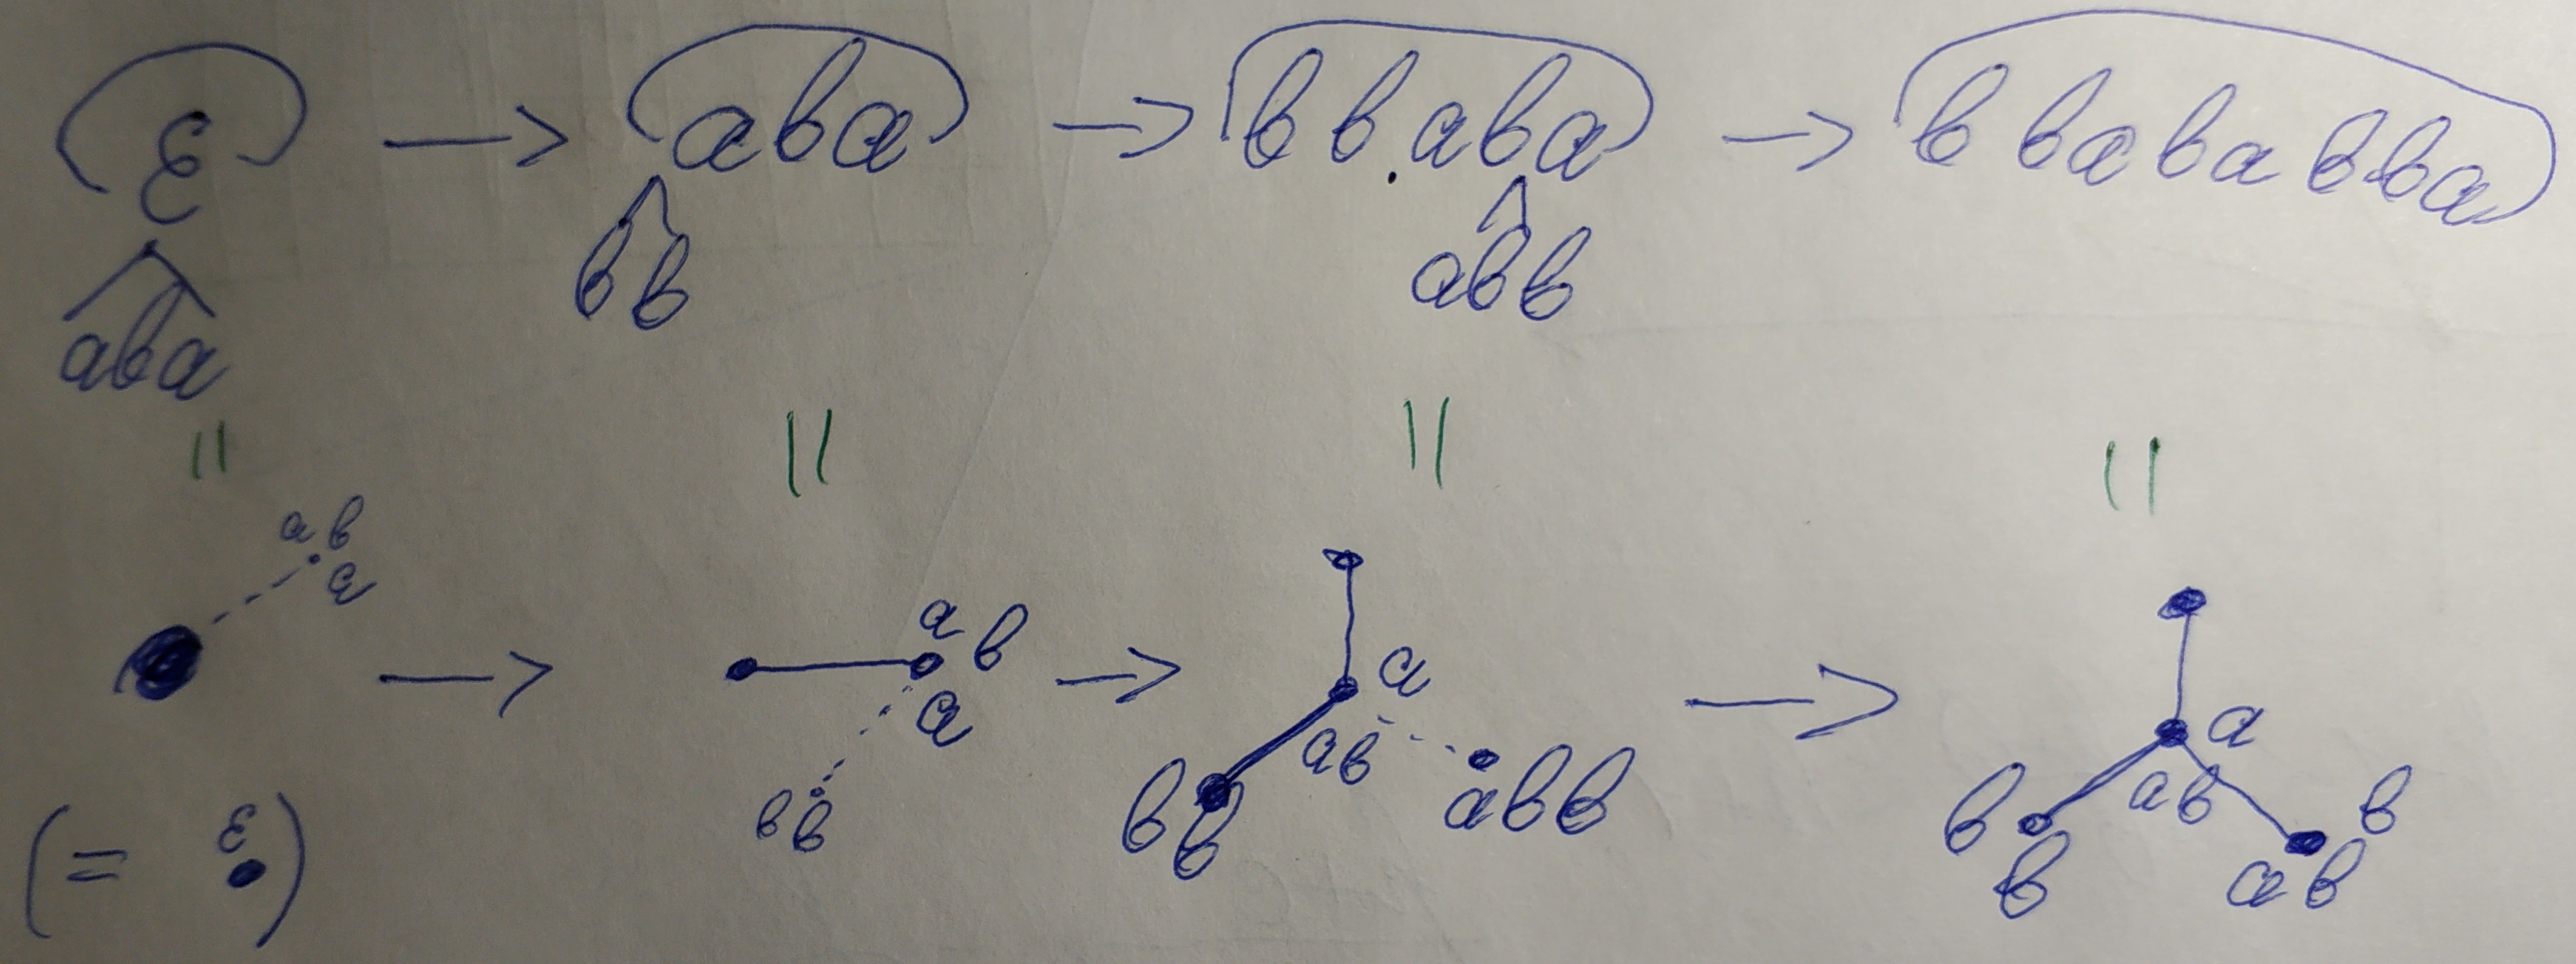
\includegraphics[height=5cm]{TI-HW-006-6.jpg}
                                \caption{Процесс генерации слов и его представление в виде наращивания дерева.}
                            \end{figure}

                            Давайте рисовать деревья на плоскости, в каждой вершине внешней грани которой напишем по слову. Будем строить такие графы для каждого слова следующим образом, что каждый раз при обходе периметра графа по часовой стрелке мы будем читать наше слово. Сначала возьмём вершину, на которой ничего не написано; такой граф соответствует представление $\varepsilon$. Затем когда мы вставляем в наше слово слово $w$, то будем рисовать новую вершину (для $w$). На старом графе найдём угол и место в написанном в нём слове, в котором находится место желанной вставки (точнее, может находиться: например, если в третьем графе на картинке вставлять слово в промежуток $bb \text{\textvisiblespace} aba$, то его можно вставить либо в вершину со словом $abb$ слева от $abb$, либо в $bb$ справа от $bb$), и соединим новую вершину с данной вершиной так, чтобы новое ребро делило найденное слово в указанном месте (см. рис. выше). На новой вершине в единственном угле напишем слово $w$. При этом начальную пустую вершину можно (но лучше стоит) удалить.

                            Заметим тогда, что на каждой вершине (если убрать рёбра) написано слово, которое мы вставляли, а на всём дереве (при том же обходе по часовой) полученное соответствующими операциями вставки зацикленное слово.
                            
                            \begin{figure}[H]
                                \centering
                                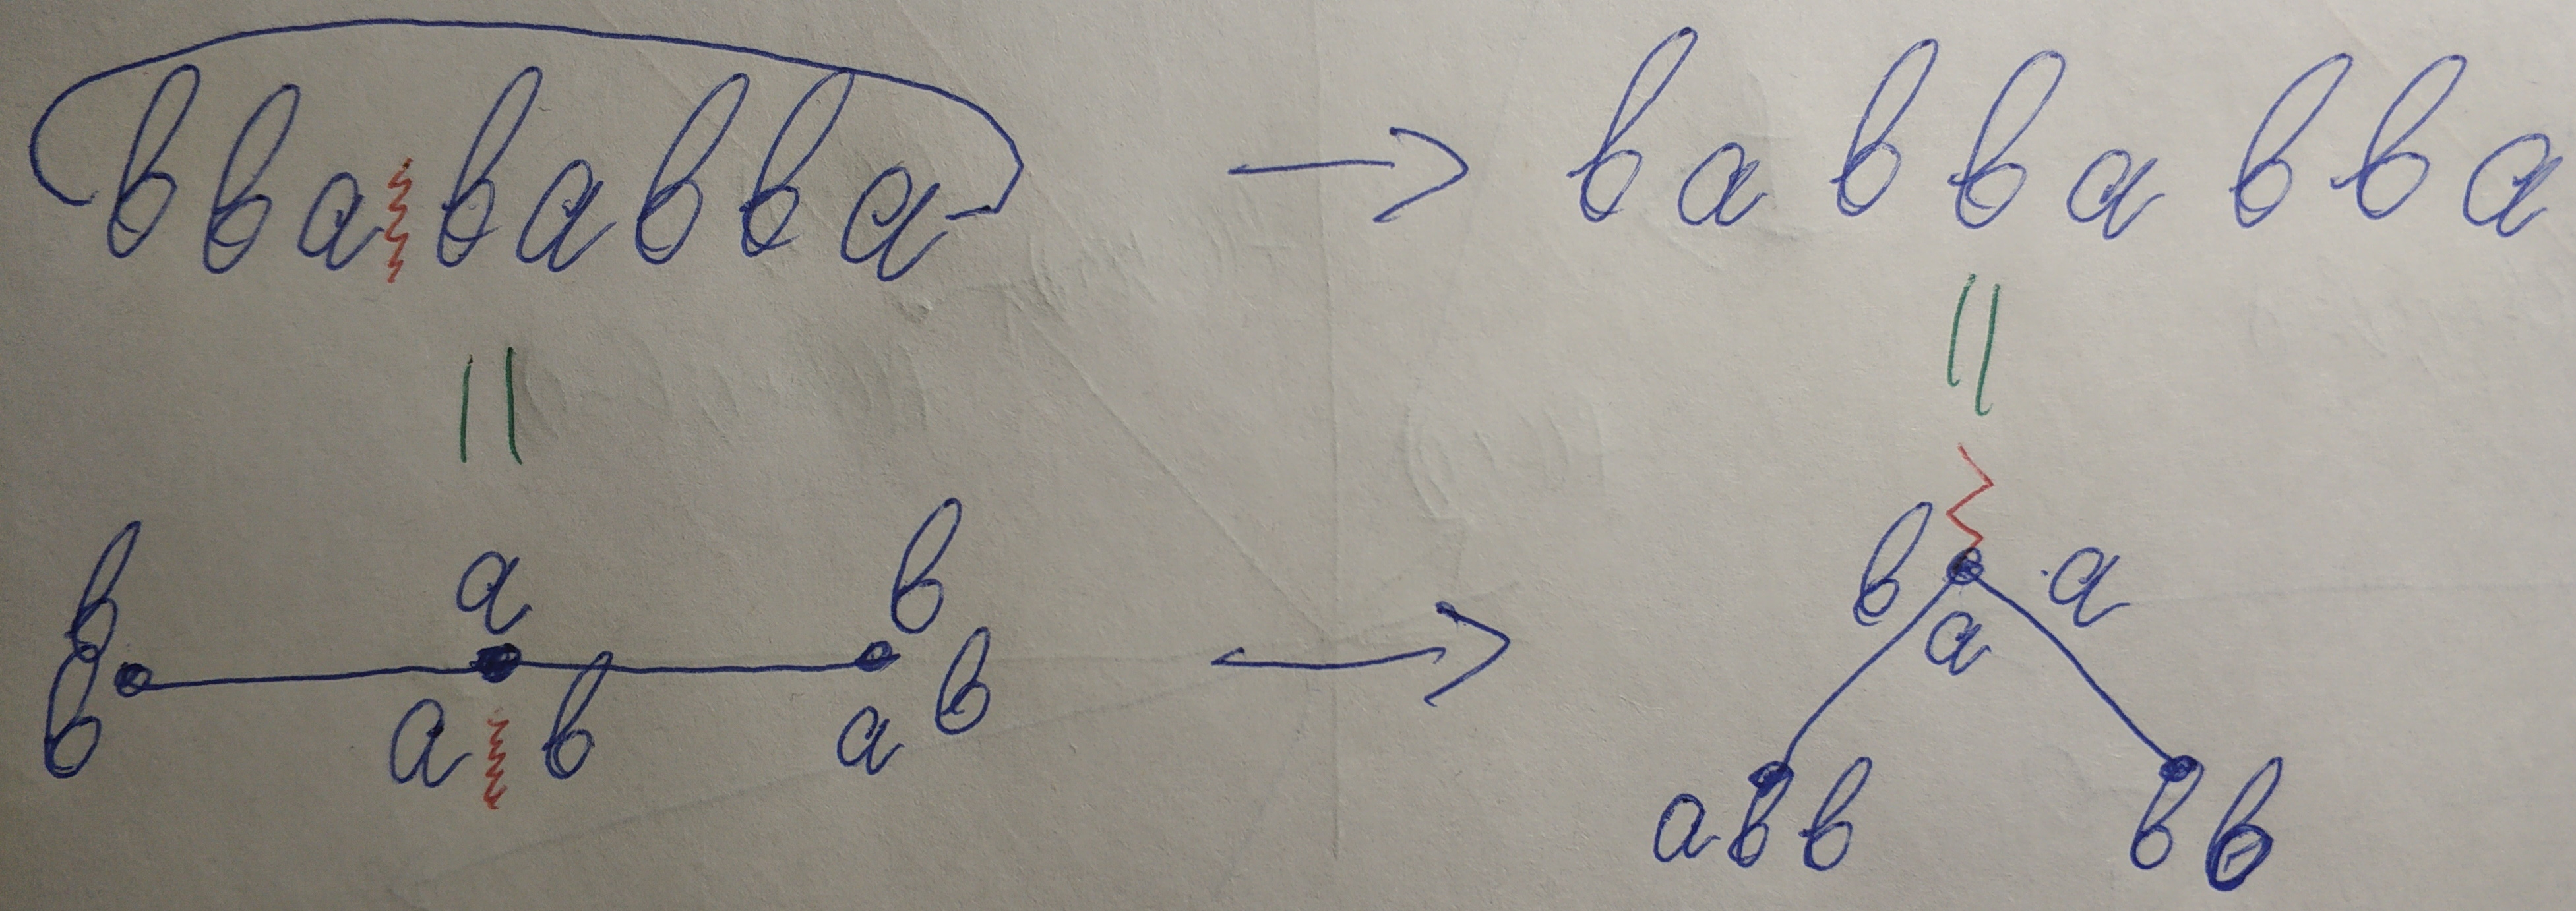
\includegraphics[height=5cm]{TI-HW-006-7.jpg}
                                \caption{Превращение дерева зацикленного слова в дерево разорванного слова.}
                            \end{figure}
                            
                            Теперь найдём на этом графе место, где нужно разорвать слово (опять же любое место), протянем через место от выбранной вершины ребро в бесконечность вверх и подвесим всё дерево за эту вершину. Тогда можно считать, что на каждой вершине снизу написано слово из $M$, а в некоторых промежутках между буквами в этих словах спускаются вниз рёбра к другим вершинам. При этом слова в вершинах являются циклическими сдвигами изначальных слов, но так как $M$ устойчив к циклическим сдвигам, то можно всё ещё говорить, что это слова из $M$. Тогда полученное слово может быть получено просто написанием сначала слова вершине, затем вставкой в соответствующие его места слов из вершин второго уровня, затем из третьего, из четвёртого и т.д. Т.е. данное слово лежит в $\Insertion(M)$.
                            
                        \item Рассмотрим грамматику $(\Sigma, \{S\}, R, S)$, где множество правил $R$ состоит из следующих правил. Для каждого $s_1 \dots s_n \in M$, где $s_1, \dots, s_n \in \Sigma$ напишем правило
                            \[S \to S s_1 S \dots S s_n S.\]
                            А также добавим правило $S \to \varepsilon$.

                            Покажем, что всякое $w \in L(S)$ лежит в $\Insertion(M)$, по (полной) индукции по $|w|$.

                            В дереве разбора $w$ есть вершины, где написаны терминальные символы (их обычно мы за вершины не считаем), вершины с символом $S$, у которого нет детей (он заменяется на $\varepsilon$), и вершины с символом $S$, которые заменяются на некоторое слово вида $S s_1 \dots s_n S$. Вершины первого и второго вида --- листы, поэтому вершины третьего вида образуют поддерево. Найдём в нём лист. Тогда это символ $S$, который был заменён на $S s_1 \dots s_n S$, где потом каждый $S$ бвл заменён на $\varepsilon$. Тогда вместо этой замены ($S \to S s_1 \dots s_n S$) сделаем замену $S \to \varepsilon$. Тогда дерево уменьшилось, полученное слово $w'$ меньше $w$, и по предположению индукции $w' \in \Insertion(M)$. Тогда возвращая дерево в изначальный вид, мы вставляем в $w'$ в некоторое место $s_1 \dots s_n$, т.е. $w \in \Insertion(M)$.

                            Теперь покажем, что всякое $w \in \Insertion(M)$ лежит в $L(S)$, по (полной) индукции по $|w|$.

                            Если $w$ пусто, то $w \in \Insertion(M)$. Иначе оно получается из какого-то слова $w' \in \Insertion(M)$ вставлением строчки $s_1 \dots s_n$ в некоторое место. По предположению индукции $w' \in L(S)$. Тогда рассмотрим дерево разбора. Найдём в нём место, где мы хотели вставить $s_1 \dots s_n$. Найдём там вершину $S$. И вместо замены $S \to \varepsilon$ навесим на неё замену $S \to S s_1 \dots s_n S$, где на каждое $S$ навесим замену $S \to \varepsilon$. Тогда получим дерево разбора $w$, т.е. $w \in L(S)$.

                            Следовательно грамматика задаёт то, что нужно.
                    \end{enumerate}
                \end{proof}

                \begin{corollary}\ 
                    \begin{enumerate}
                        \item $L(\{q_1; q_2\}^*) = \Insertion(L(S))$ для некоторого конечного $S \subseteq \{q_1; q_2\}^*$.
                        \item $L(\{q_1; q_2\}^*)$ задаётся грамматикой.
                    \end{enumerate}
                \end{corollary}

                \begin{proof}
                    $L(S)$ конечен и замкнут относительно циклических сдвигов символов (даже относительно перестановок символов).
                    \begin{enumerate}
                        \item Поскольку $L(\{q_1; q_2\}^*)$ замкнут относительно циклических сдвигов символов (даже относительно перестановок символов), то
                            \[L(\{q_1; q_2\}^*) = L(L^\circ(\{q_1; q_2\}^*)) = L(\Insertioncirc(L(S))) = \Insertion(L(S)).\]
                        \item $L(\{q_1; q_2\}^*) = \Insertion(L(S))$ задаётся грамматикой.
                    \end{enumerate}
                \end{proof}
        \end{enumerate}
    \end{problem}
\end{document}